%%%%%%%%%%%%%%%%%%%%%%%%%%%%%%%%%%%%%%%%%
% Wenneker Assignment
% LaTeX Template
% Version 2.0 (12/1/2019)
%
% This template originates from:
% http://www.LaTeXTemplates.com
%
% Authors:
% Vel (vel@LaTeXTemplates.com)
% Frits Wenneker
%
% License:
% CC BY-NC-SA 3.0 (http://creativecommons.org/licenses/by-nc-sa/3.0/)
% 
%%%%%%%%%%%%%%%%%%%%%%%%%%%%%%%%%%%%%%%%%

%----------------------------------------------------------------------------------------
%	PACKAGES AND OTHER DOCUMENT CONFIGURATIONS
%----------------------------------------------------------------------------------------

\documentclass[11pt, parskip=half]{scrartcl} % Font size

%%%%%%%%%%%%%%%%%%%%%%%%%%%%%%%%%%%%%%%%%
% Wenneker Assignment
% Structure Specification File
% Version 2.0 (12/1/2019)
%
% This template originates from:
% http://www.LaTeXTemplates.com
%
% Authors:
% Vel (vel@LaTeXTemplates.com)
% Frits Wenneker
%
% License:
% CC BY-NC-SA 3.0 (http://creativecommons.org/licenses/by-nc-sa/3.0/)
% 
%%%%%%%%%%%%%%%%%%%%%%%%%%%%%%%%%%%%%%%%%

%----------------------------------------------------------------------------------------
%	PACKAGES AND OTHER DOCUMENT CONFIGURATIONS
%----------------------------------------------------------------------------------------

\usepackage{amsmath, amsfonts, amsthm} % Math packages

\usepackage{geometry}

\usepackage{listings} % Code listings, with syntax highlighting

\usepackage[french]{babel} % English language hyphenation

\usepackage{graphicx} % Required for inserting images
\graphicspath{{Figures/}{./}} % Specifies where to look for included images (trailing slash required)

\usepackage{booktabs} % Required for better horizontal rules in tables

\usepackage{subcaption} % Required for creating figures with multiple parts (subfigures)

\usepackage{todonotes} % Required for inserting todo notes

\usepackage{array} % Required for customising tables

\usepackage{hyperref} % Required for adding links	and customising them

\numberwithin{equation}{section} % Number equations within sections (i.e. 1.1, 1.2, 2.1, 2.2 instead of 1, 2, 3, 4)
\numberwithin{figure}{section} % Number figures within sections (i.e. 1.1, 1.2, 2.1, 2.2 instead of 1, 2, 3, 4)
\numberwithin{table}{section} % Number tables within sections (i.e. 1.1, 1.2, 2.1, 2.2 instead of 1, 2, 3, 4)

\setlength\parindent{0pt} % Removes all indentation from paragraphs

\usepackage{enumitem} % Required for list customisation
\setlist{noitemsep} % No spacing between list items

%----------------------------------------------------------------------------------------
%	DOCUMENT MARGINS
%----------------------------------------------------------------------------------------

\usepackage{geometry} % Required for adjusting page dimensions and margins

\geometry{
	paper=a4paper, % Paper size, change to letterpaper for US letter size
	top=2.5cm, % Top margin
	bottom=3cm, % Bottom margin
	left=3cm, % Left margin
	right=3cm, % Right margin
	headheight=0.75cm, % Header height
	footskip=1.5cm, % Space from the bottom margin to the baseline of the footer
	headsep=0.75cm, % Space from the top margin to the baseline of the header
	%showframe, % Uncomment to show how the type block is set on the page
}

%----------------------------------------------------------------------------------------
%	FONTS
%----------------------------------------------------------------------------------------

\usepackage[utf8]{inputenc} % Required for inputting international characters
\usepackage[T1]{fontenc} % Use 8-bit encoding

\usepackage{fourier} % Use the Adobe Utopia font for the document

%----------------------------------------------------------------------------------------
%	SECTION TITLES
%----------------------------------------------------------------------------------------

\usepackage{sectsty} % Allows customising section commands

\sectionfont{\vspace{6pt}\centering\normalfont\scshape} % \section{} styling
\subsectionfont{\normalfont\bfseries} % \subsection{} styling
\subsubsectionfont{\normalfont\itshape} % \subsubsection{} styling
\paragraphfont{\normalfont\scshape} % \paragraph{} styling

%----------------------------------------------------------------------------------------
%	HEADERS AND FOOTERS
%----------------------------------------------------------------------------------------

\usepackage{scrlayer-scrpage} % Required for customising headers and footers

\ohead*{} % Right header
\ihead*{} % Left header
\chead*{} % Centre header

\ofoot*{} % Right footer
\ifoot*{} % Left footer
\cfoot*{\pagemark} % Centre footer
 % Include the file specifying the document structure and custom commands
\geometry{a4paper, margin=0.65in, footskip=25pt}

%----------------------------------------------------------------------------------------
%	TITLE SECTION
%----------------------------------------------------------------------------------------

\title{	
	\normalfont\normalsize
	\large\textsc{Sorbonne Université, UFR de Physique}\\ % Your university, school and/or department name(s)
	\vspace{2pt} % Whitespace
	\normalsize Master 1 : Physique fondamentale et applications\\
	\vspace{25pt} % Whitespace
	\rule{\linewidth}{0.5pt}\\ % Thin top horizontal rule
	\vspace{20pt} % Whitespace
	{\huge Projet IA : Le Modèle d'Ising}\\ % The assignment title
	\vspace{2pt} % Whitespace
	{Intelligence artificielle pour la physique}\\
	\vspace{12pt} % Whitespace
	\rule{\linewidth}{2pt}\\ % Thick bottom horizontal rule
	\vspace{12pt} % Whitespace
}

\author{\LARGE A. Cremel-Schlemer \large (3800159) \\ \LARGE G. Carvalho \large (28709594) \\ \LARGE M. Panet \large (28705836)} % Your name

\date{\normalsize\today} % Today's date (\today) or a custom date

\begin{document}

\maketitle % Print the title
\tableofcontents % Print the contents

\newpage

\addcontentsline{toc}{section}{Introduction}
\section*{Introduction}

Le modèle d'Ising est un modèle de physique statistique introduit par Rudolph Peierls, Wilhelm Lenz et Ernst Ising dans les années 1920. Malgré sa remarquable simplicité, ce modèle permet de mettre en évidence un comportement de transition de phase.

Sous sa formulation historique, le modèle d'Ising permet d'étudier la transition de phase paramagnétique/ferromagnétique d'un matériau. Certains matériaux, appelés ferromagnétiques, possèdent une aimantation intrinsèque, comme les aimants. Cette propriété découle d'interactions à courte portée entre les spins d'un cristal. Cependant, le physicien Pierre Curie a découvert en 1895 que ces matériaux perdent leur propriété magnétique au-dessus d'une température caractéristique appelée température de Curie, notée $T_C$.

Il existe également des matériaux paramagnétiques, qui ne sont pas magnétiques à l'origine mais le deviennent en présence d'un champ magnétique extérieur puissant. En l'absence de champ magnétique extérieur, les spins de ces matériaux sont désordonnés, conduisant à un moment magnétique moyen nul, rendant le matériau non magnétique. Sous l'action d'un champ magnétique extérieur, ces moments se polarisent, rendant le matériau magnétique.

L'hamiltonien du modèle d'Ising prend donc en compte ces deux propriétés, avec une partie relative à l'interaction ferromagnétique à courte portée et une autre relative à l'interaction de chaque spin du cristal avec un champ magnétique extérieur. Dans la plupart des modèles numériques, on travaille sans champ extérieur.

La généralité du modèle d'Ising, avec ses interactions locales et l'interaction individuelle avec une force extérieure, transcende la physique et permet de décrire qualitativement et parfois quantitativement une grande variété de situations (paramagnétisme, gaz réticulaire, agents économiques, modèles écologiques, analyse et traitement de l'image). Il a même donné lieu à un modèle plus général : le modèle de Potts, qui généralise l'aspect binaire du modèle d'Ising lié à la binarité des spins.

À travers notre exposé sur l'intelligence artificielle, nous allons nous intéresser à un jeu de données constitué de 16,000 images issues d'une simulation numérique du modèle d'Ising 2D. Chaque image est associée à une température caractéristique allant de $0.25$ à $4$ (sans unité) et à un label. Le label renseigne sur la phase dans laquelle l'image se trouve. La \textit{phase ferromagnétique} est une phase où les spins sont globalement tous alignés ou forment des îlots de spins alignés ($|M| > 0$). Le label \textit{phase paramagnétique} rend compte du régime où les spins sont globalement désordonnés ($M = 0$).

Nous allons explorer différentes méthodes pour voir quelles solutions d'intelligence artificielle nous permettent de déterminer, à partir d'une image donnée, si l'on est dans la phase paramagnétique ou ferromagnétique. Nous nous intéresserons également à la manière dont sont générées les données du modèle d'Ising. Nous chercherons à voir s'il est possible de prédire la température d'une image de manière fiable et même s'il est possible de générer de nouvelles données sans faire appel à une simulation numérique coûteuse.

\newpage
\section{Génération de données}

Afin de mieux cerner le problème initial, nous avons recréé la simulation du modèle d'Ising 2D pour des images de dimensions $40 \times 40$, comme celle présente dans le dataset.

\subsection{Théorie, Hypothèses et Hamiltonien}
Le modèle d'Ising 2D est une approche numérique du problème posé en introduction, où l'on fait l'hypothèse d'un cristal ferromagnétique plat et de maille carrée pour lequel chaque atome est associé à un pixel d'une image.

Chaque spin est représenté soit par un 0, soit par un 1, où le 1 correspond à un spin "Up" et le 0 à un spin "Down". Afin d'améliorer la validité du modèle et de surmonter les problèmes potentiels aux extrémités des images, des conditions aux bords périodiques sont utilisées. Concrètement, cela revient à considérer la surface d'un tore que l'on aurait déplié (cf. Figure \ref{fig:ising2D}).

\begin{figure}[h]
	\begin{subfigure}{0.5\textwidth}
		\centering
		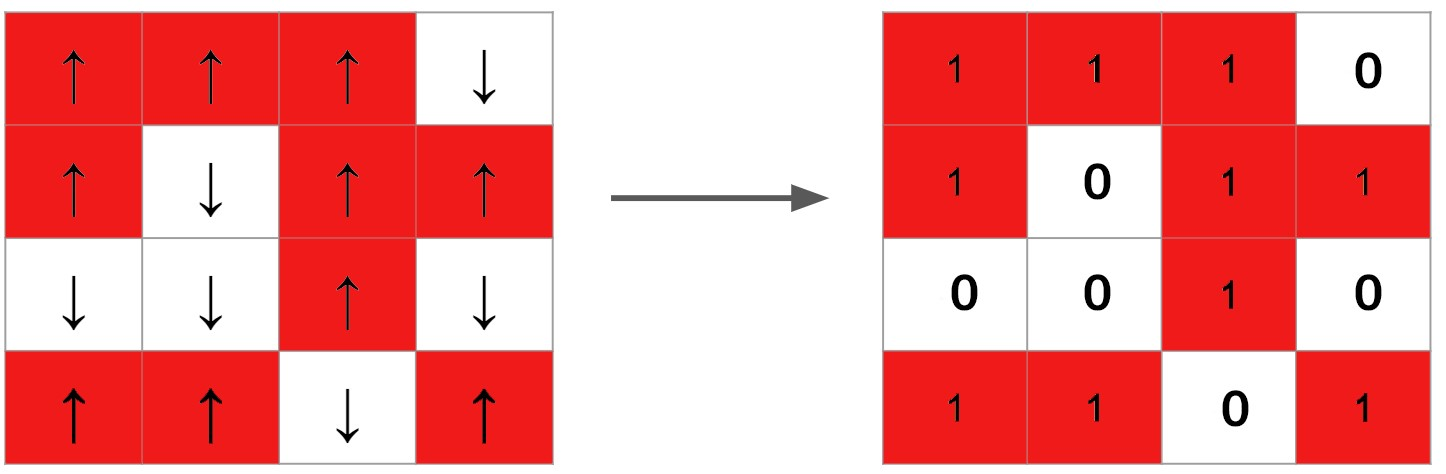
\includegraphics[width=0.95\linewidth]{./figures/torus_left.jpg}
		\caption{Les spins sont soit Up = 1, soit Down = 0}
	\end{subfigure}
	\begin{subfigure}{0.5\textwidth}
		\centering
		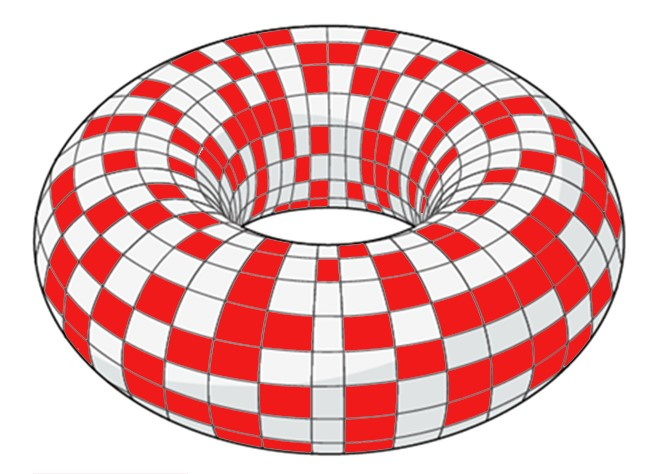
\includegraphics[width=0.5\linewidth]{./figures/torus_right.jpg}
		\caption{Conditions aux bords périodiques}
	\end{subfigure}
	\caption{Représentation du modèle d'Ising 2D}
	\label{fig:ising2D}
\end{figure}


Le hamiltonien du problème est donné par l'équation :


\begin{equation*}
	H = -J  \displaystyle \sum_{i,j}\sigma_{i}\sigma_{j} - h\displaystyle \sum_{i} \sigma_{i}
\end{equation*}

où $\sigma_{i} = \pm 1$. Cela dit, comme nous travaillons avec des $0$ et des $1$, il y a quelques manipulations à réaliser sur l'hamiltonien pour transformer les opérations de sorte que $\sigma_{i}$ puisse prendre soit la valeur 0 soit la valeur 1.

Comme nous cherchons à mettre en évidence la façon dont un matériau ferromagnétique perd brutalement sa magnétisation en fonction de sa température, il devient clair que l'on ne s'intéresse pas à la deuxième partie de l'hamiltonien qui nous renseigne sur la manière dont les spins s'alignent avec un champ magnétique extérieur.

Il ne nous reste donc qu'à traiter :
\begin{equation*}
	H = -J  \displaystyle \sum_{i,j}(2\sigma_{i}-1)(2\sigma_{j}-1)
\end{equation*}
Avec $\sigma_{i} \in \{0,1\}$

Que signifie cet Hamiltonien ? C'est un Hamiltonien de couplage entre spins. Il est responsable du ferromagnétisme du matériau. À priori, pour respecter la physique du système que l'on cherche à étudier, ce couplage ne se réalise qu'à courte portée, entre particules identiques, ici le spin. Les spins "plus proches voisins" subissent alors une interaction d'échange à courte portée $\pm J$. Par simplicité et pour garder l'aspect très général de l'algorithme, on choisit de travailler avec des constantes adimensionnées de sorte que : $\frac{J}{K_B} = 1$.

\subsection{Agitation thermique et probabilité}
Nous allons maintenant nous approcher d'un des spins de notre modèle. Situé au centre, ses plus proches voisins forment une croix suisse autour de lui. Calculons maintenant son Hamiltonien local :

\begin{equation*}
	H_{local} = E_{ij} =  (2\sigma_{i}-1) \displaystyle \sum_{j}(2\sigma_{j}-1) = (2\sigma_{i}-1) \times \bigg[ 2\times( R + L + U + D ) -4 \bigg]
\end{equation*}
avec :

\begin{figure}[h]
	\centering
	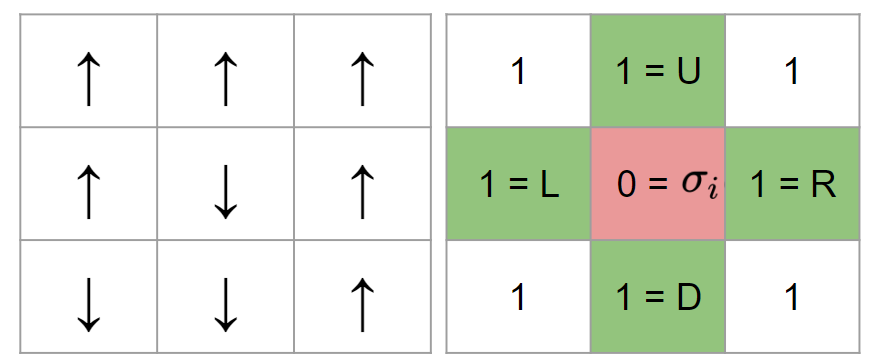
\includegraphics[width=0.5\linewidth]{./figures/H.png}
	\caption{Hamiltonien local}
	\label{fig:H}
\end{figure}

Partons d'un système idéal où tous les spins sont alignés. En raison de l'agitation thermique, un spin aléatoire du cristal inverse son sens. La variation d'énergie associée à ce changement est donnée par :

\begin{equation*}
	\Delta E = E_f - E_i
\end{equation*}

Et la probabilité qu'un tel changement s'opère est proportionnelle au poids de Boltzmann :

\begin{equation*}
	P(\Delta E) \propto e^{-\beta \Delta E} \propto e^{-\frac{\Delta E}{T}}
\end{equation*}

L'idée est la suivante : l'ordinateur va piocher une case au hasard, calculer le $\Delta E$ associé. Ce $\Delta E$ ne peut prendre que 5 valeurs possibles :

\begin{center}
	\begin{tabular}{|l|m{4cm}|}
		\hline
		n voisin de sens opposé & $\Delta E $ \\
		\hline
		0                       & 8           \\
		1                       & 4           \\
		2                       & 0           \\
		3                       & -4          \\
		4                       & -8          \\\hline
	\end{tabular}
\end{center}

\vspace{4mm}

Dans le cas où $\Delta E \in {0, -4, -8}$, l'énergie est minimisée, et donc le changement s'opère naturellement : l'ordinateur modifie le pixel d'état. Dans le cas inverse, c'est-à-dire lorsque $\Delta E \in {4, 8}$, un nombre aléatoire $x$ est tiré selon une distribution uniforme entre 0 et 1 et est comparé à $e^{-\frac{\Delta E}{T}}$. Si $x < e^{-\frac{\Delta E}{T}}$, alors l'ordinateur modifie le pixel d'état ; sinon, il ne le fait pas.

Nous remarquons que plus $T$ est élevée, plus la probabilité de transition est importante.

On peut alors lancer la simulation. Pour une température fixée, nous réalisons un certain nombre de tentatives de changement de spin. Le système va se relaxer jusqu'à atteindre un équilibre, où la moyenne des spins composant l'image est stable après chaque tentative successive de changement de l'état d'un spin de l'image.

\begin{figure}[h]
	\begin{subfigure}[c]{0.5\textwidth}
		\centering
		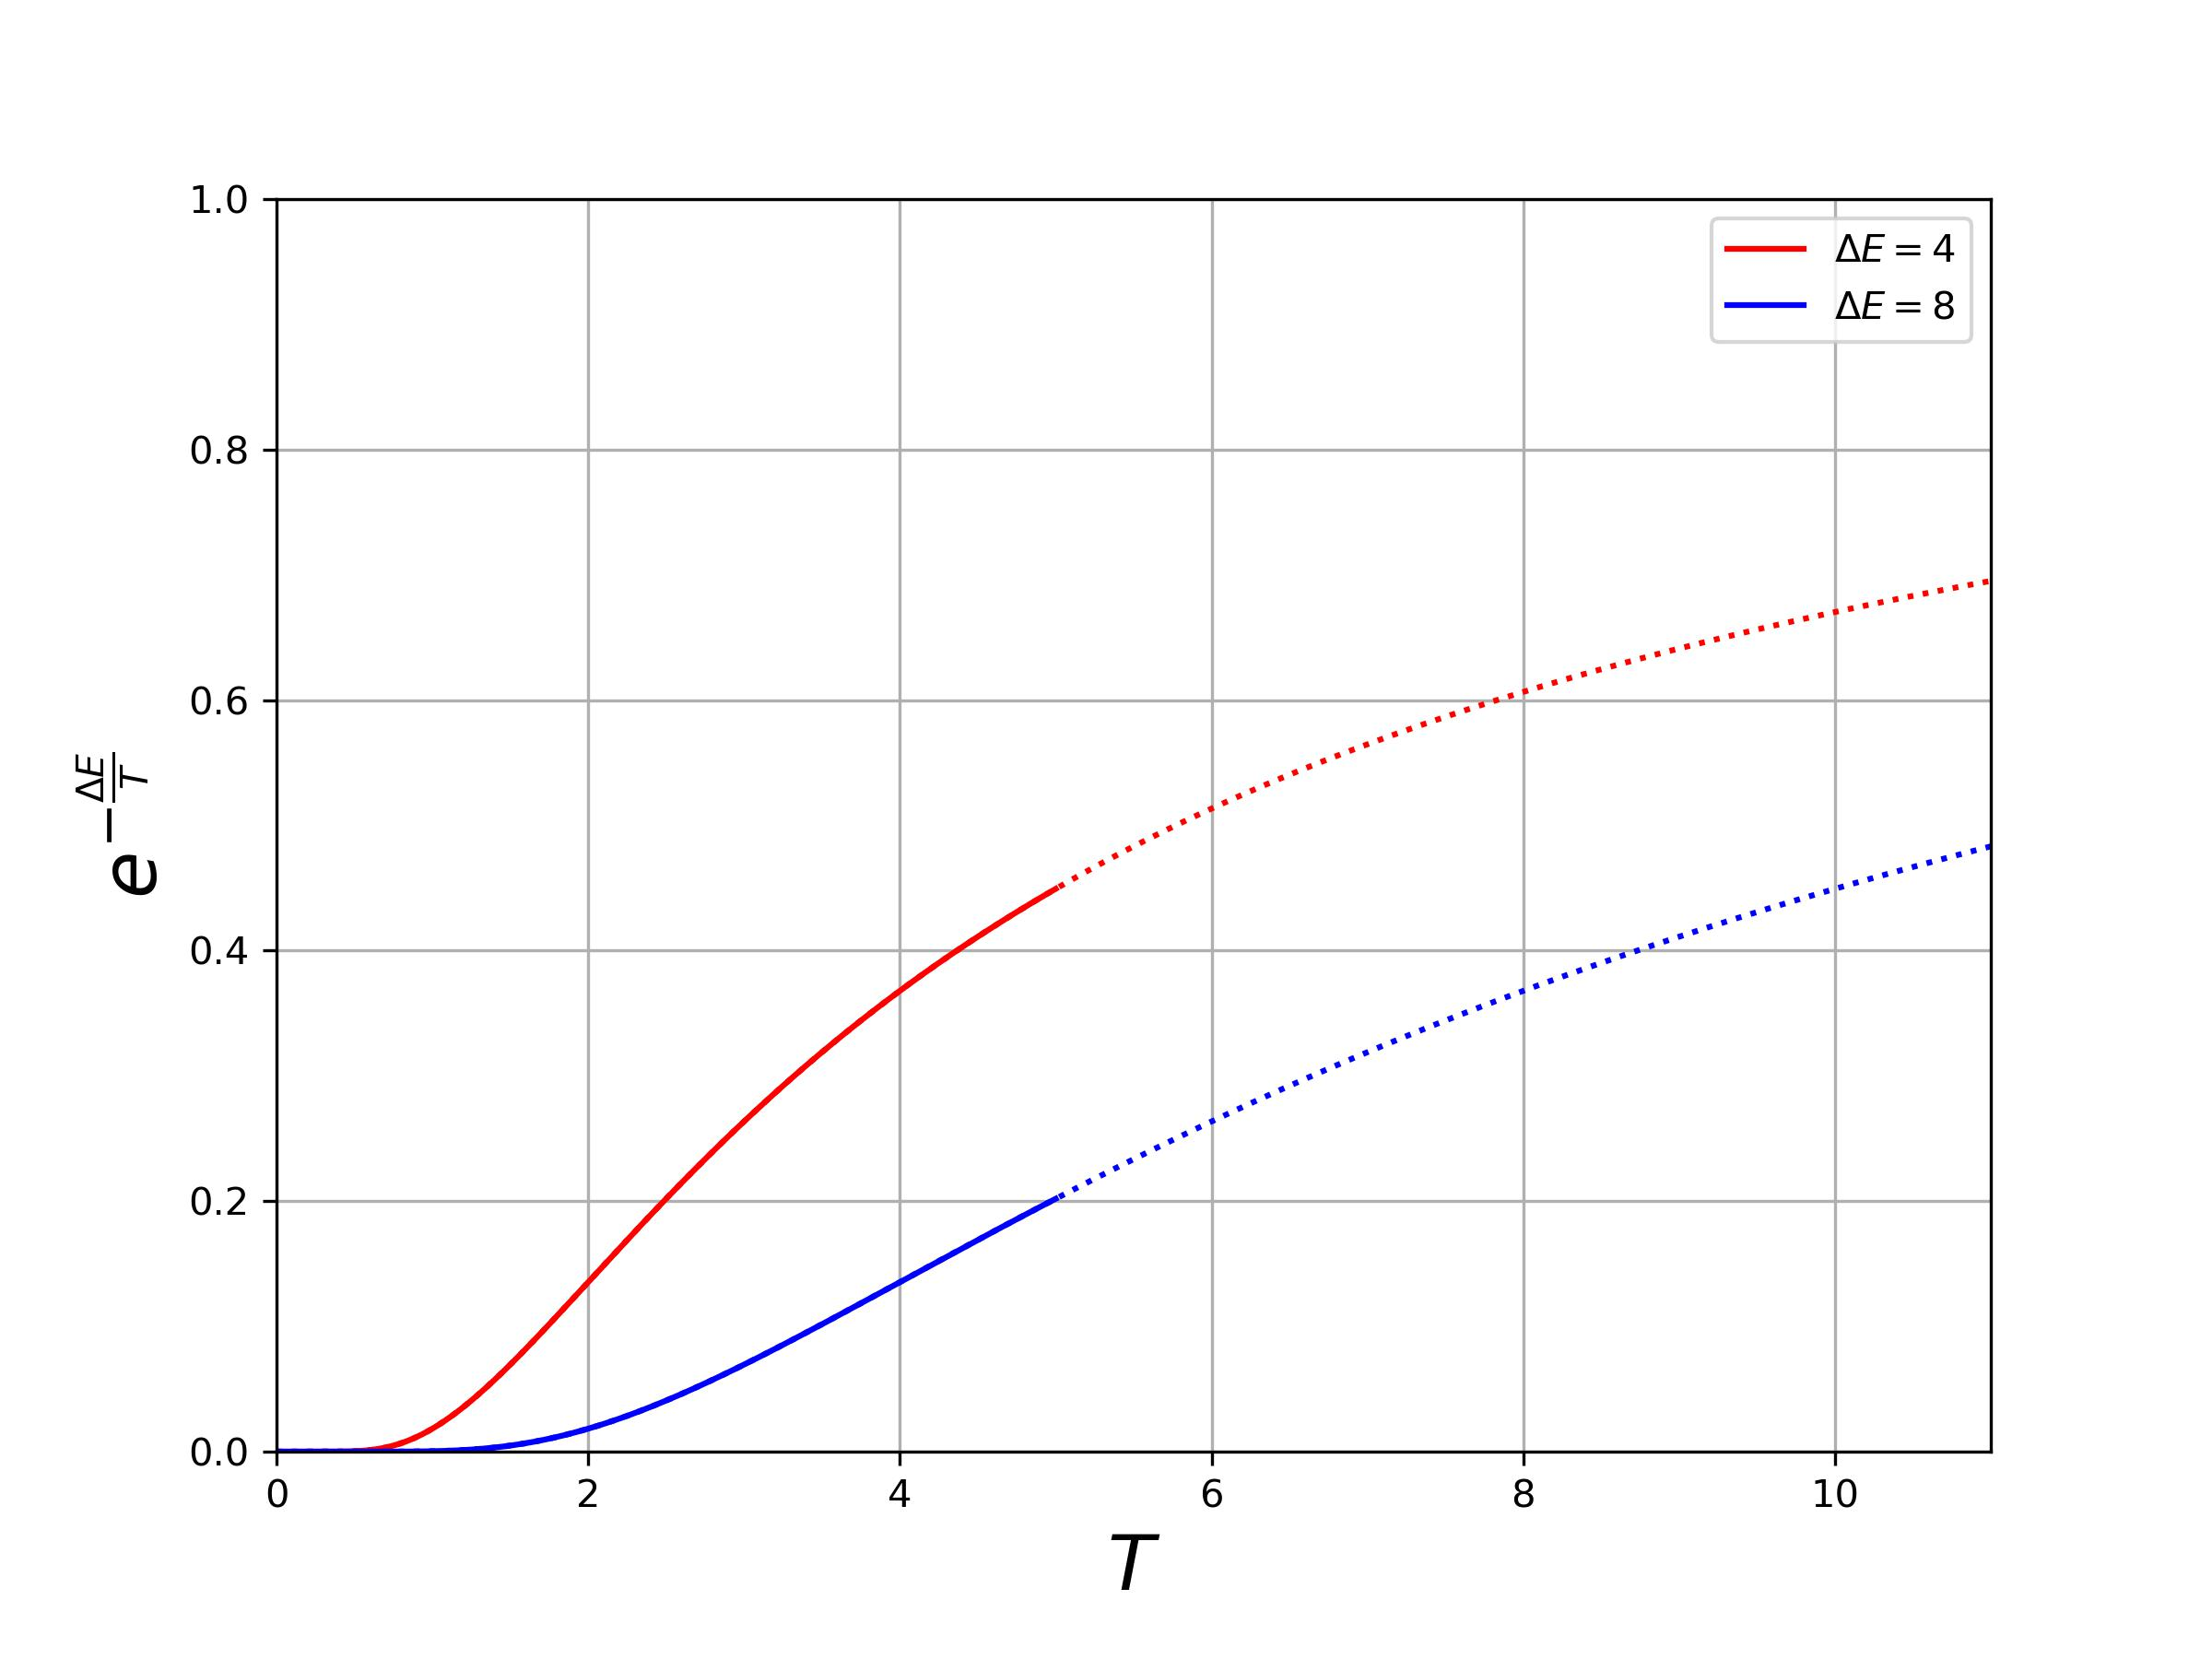
\includegraphics[width=0.95\linewidth]{./figures/proba.jpg}
		\caption{probabilité de transition en fonction de la température}
		\label{fig:H}
	\end{subfigure}
	\begin{subfigure}[c]{0.5\textwidth}		
		\centering
		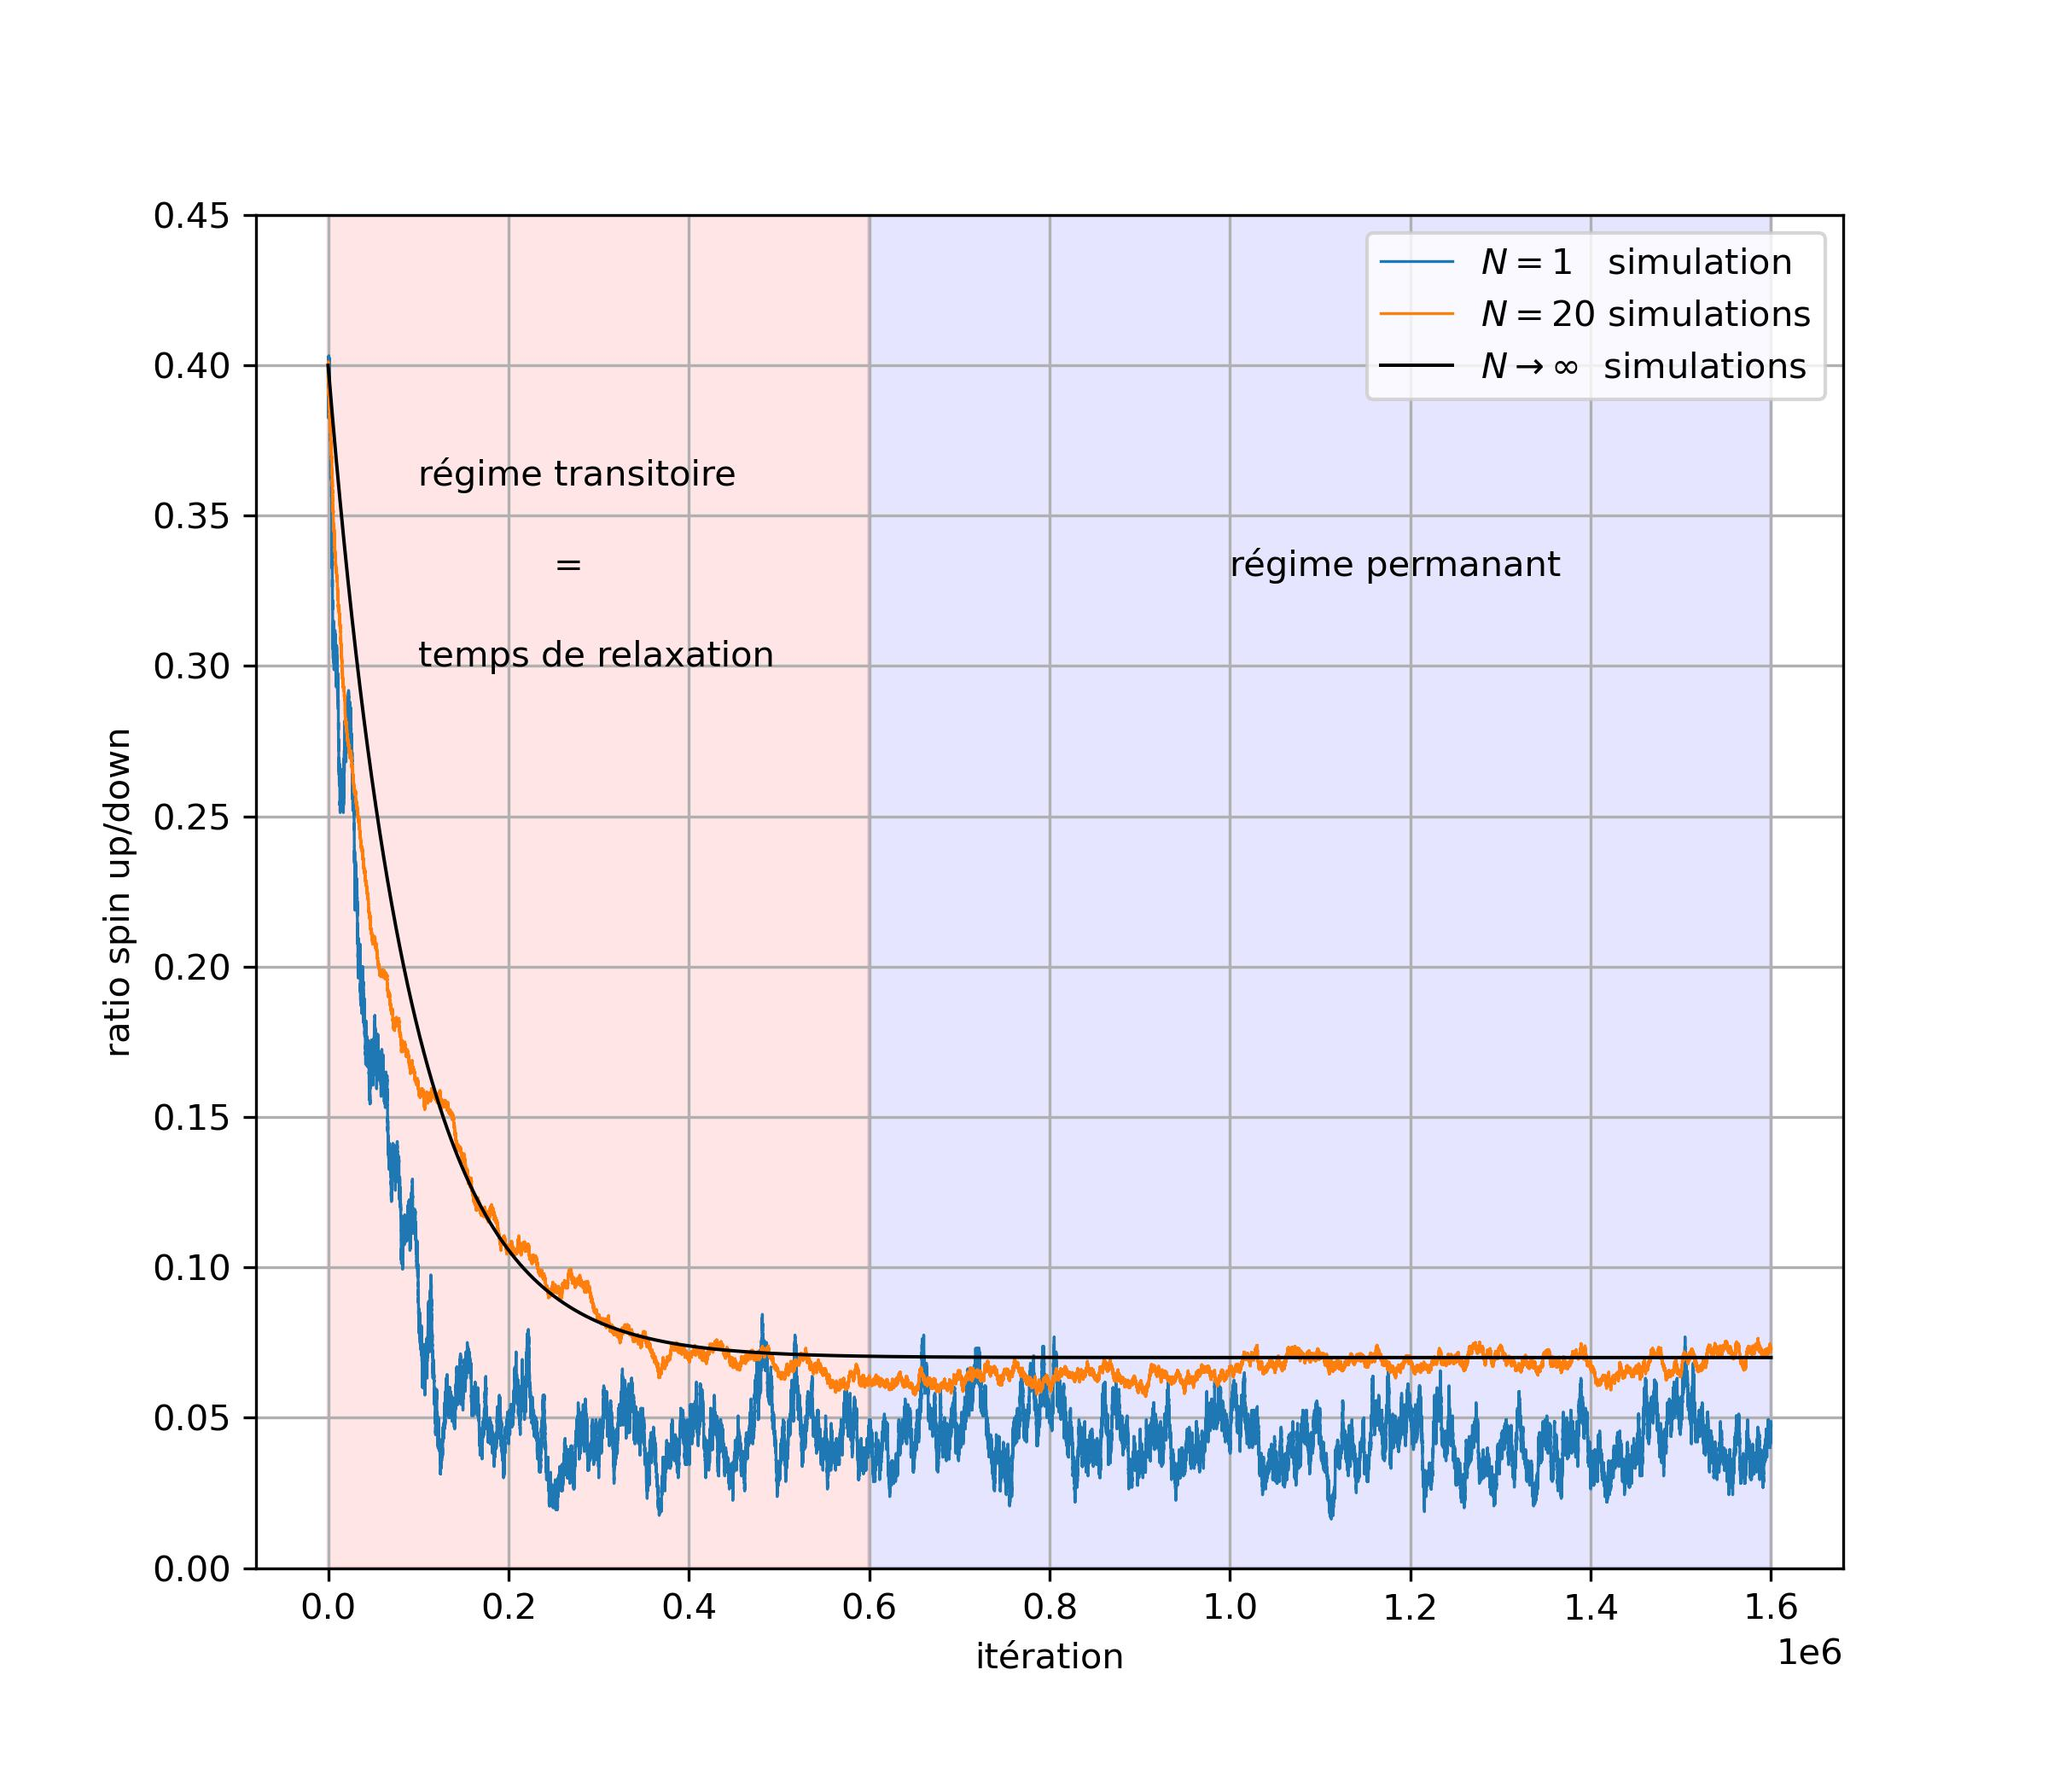
\includegraphics[width=0.95\linewidth]{./figures/simulation_ising.jpg}
		\caption{Évolution du ratio spin up/spin down pour $T=2$ et $1,6$ million d'itérations.}
		\label{fig:H}
	\end{subfigure}
	\caption{}
\end{figure}

\subsection{Stabilité, cohérence de la solution et considérations techniques}

Pour chaque température, le temps de relaxation du système est plus ou moins long et il est également influencé par la composition du système de départ. Dans le cas où l'on aurait une situation initiale avec que des spins alignés, le temps de relaxation vers l'équilibre pour T proche de 0 est très rapidement trouvé car le système est déjà à l'équilibre. Le matériau est bien ferromagnétique : $\frac{|M|}{M_{max}} > 0$.

En revanche, pour T proche de 0 et un système de départ homogène avec autant de 0 que de 1, le temps de relaxation est plus lent et fait apparaître de nouveaux états d'équilibre. Les spins peuvent tous s'aligner dans un sens ou dans un autre. Il existe une autre formation, de moment magnétique total nul où il y a coexistence d'une bande up et d'une bande down. Avec l'analogie du tore, c'est comme si on avait trempé un donut dans du chocolat jusqu'à la moitié. C'est une situation qui se rapproche de la situation dite d'antiferromagnétisme \cite{ferromag}.

\begin{figure}[h]
	\centering
	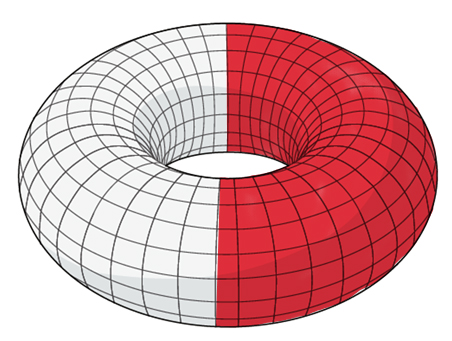
\includegraphics[width=0.3\linewidth]{./figures/donut.jpg}
	\caption{Artefact à basse température $M=0$}
	\label{fig:H}
\end{figure}

Pour éviter des situations non souhaitées, nous initialisons la simulation avec un ratio de 0.25\% ou 0.75\% de 1. Cela facilite la convergence vers un état d'équilibre dans les basses et les hautes températures et limite l'apparition de figures intermédiaires qui ne correspondraient pas à la physique que l'on cherche à mettre en avant (ferromagnétisme).

Le temps de calcul avec un algorithme non optimisé écrit en Python est lent. Générer 160,000 nouvelles données est très coûteux. Cela est lié à plusieurs choses. Premièrement, Python est un langage de haut niveau, intelligible par un humain mais très éloigné d'un langage machine comme l'assembleur où la nature des données est très spécifiquement choisie et traitée. En Python, il existe donc une procédure de "traduction" de l'humain vers la machine qui est coûteuse et conduit à des performances réduites. Il est possible d'optimiser le programme avec des principes généraux de réduction du nombre de calculs à effectuer pour réaliser une tâche (calcul en amont de certaines variables, etc.).

Il est aussi possible d'écrire ce même code dans un langage compilé, comme le C++, qui est un langage dit "typé", c'est-à-dire que l'utilisateur doit faire un effort pour indiquer à l'ordinateur la nature des variables avec lesquelles il travaille pour faciliter le travail de "traduction" vers un langage machine. Cela évite "l'interprétation" au moment de la compilation du programme (la "traduction") et le programme est donc généralement plus rapide.

Il est possible, en Python et en C++, d'accélérer le programme par la parallélisation de certains calculs. C'est-à-dire que l'ordinateur va exécuter la même tâche en parallèle pour gagner du temps, un peu comme si nous, humains, pouvions recopier simultanément un texte avec la main gauche et la main droite sur deux feuilles distinctes. Ici, l'ajout de nouveaux points se fait en parallèle.

Mais il y a un problème : si en parallèle, on modifie des pixels adjacents, il risque d'y avoir un conflit dans le calcul de l'énergie. Ce problème n'est pourtant pas très important dans une image 40 par 40 dès lors que le nombre d'exécutions en parallèle n'est pas trop grand. En effet, pour 16 tâches en parallèle, $16 \times 9 = 144$ pixels sont manipulés en parallèle, ce qui représente une fraction de 9\% de l'image. En approximation, on peut dire que les erreurs en énergie sont suffisamment négligeables. Nous générons les données suivantes avec cette hypothèse et cela semble plutôt correct.

\begin{figure}[h]
	\centering
	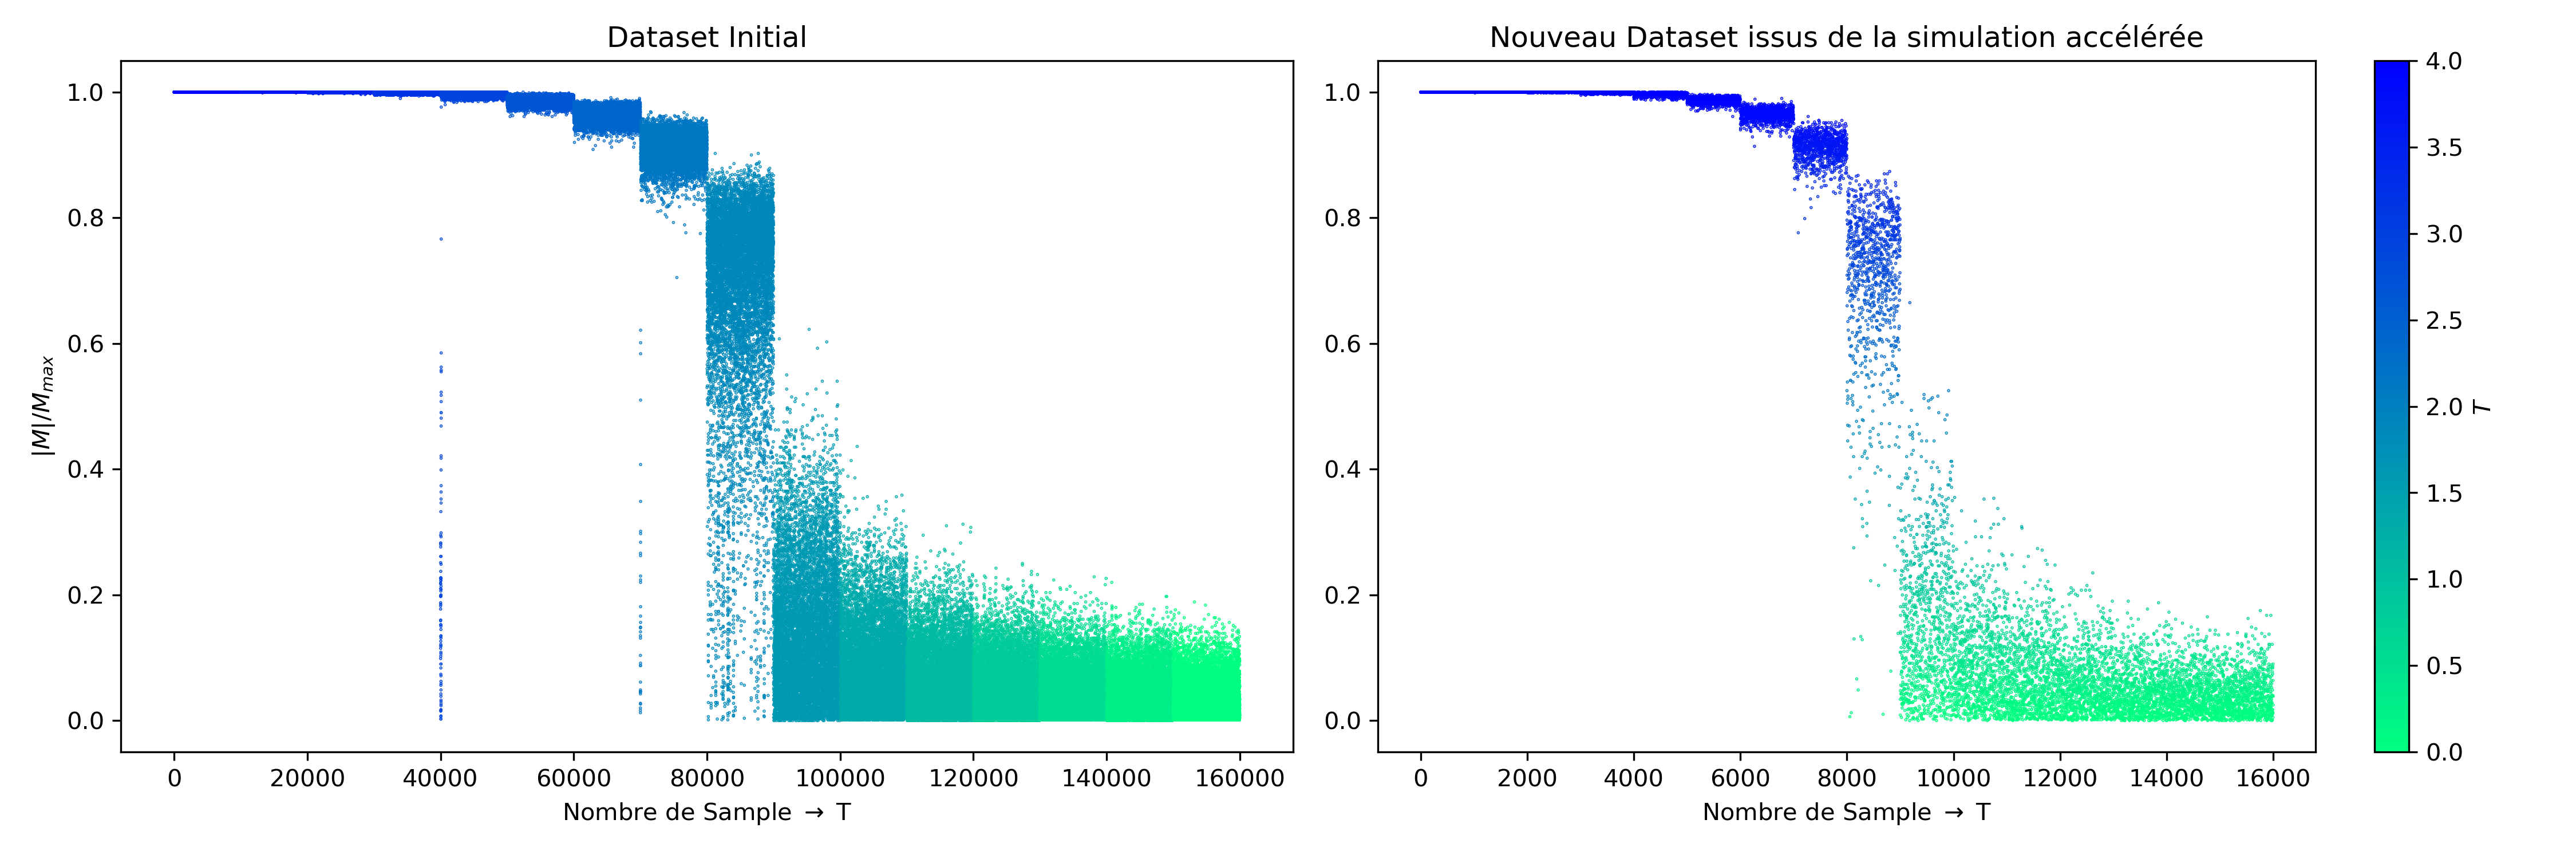
\includegraphics[width=0.95\linewidth]{./figures/new_data_compare.png}
	\caption{Nouvelles figures et comparaison avec le dataset}
	\label{fig:H}
\end{figure}

Pour prendre en compte les probabilités correctement avec la parallélisation et pour accélérer le calcul par des opérations très bas niveau, il faut se tourner vers l'algorithme de Metropolis-Hastings mis en place en 1953.

Il existe aussi une autre possibilité, celle de générer de nouvelles images avec de l'intelligence artificielle.

\section{Pré-traitement des données}
Maintenant que nous avons généré nos données, nous devons nous faire une idée de la forme de nos données afin de pouvoir les traiter de la meilleure façon possible.
Les données fournies au départ sont des vecteurs de taille $1600$ contenant des $1$ et des $0$. Ces vecteurs représentent des configurations de spins se trouvant sur une grille 2D de taille $40 \times 40$. Le dataset original est composé de $10000$ configurations de spins pour $16$ températures différentes comprises entre $0.25$ et $4.00$ avec un pas de $0.25$.
Avec ces configurations, un label est associé à chaque configuration. Ce label est une valeur binaire qui nous indique la phase dans laquelle se trouve le système.
De plus, nous avons généré un second jeu de données avec $16000$ configurations de spins pour $100$ températures comprises entre $0.25$ et $4.00$. Ce second jeu de données nous permettra de tester nos modèles sur des données avec des températures différentes de celles du jeu de données original. On pourra ainsi voir si nos modèles sont capables de se séparer des températures discrètes du jeu de données original.
Comme on peut le voir sur la figure \ref{fig:rawdata}, nos données forment un ensemble bruité mais il apparaît une symétrie par rapport à l'axe horizontal. En effet, à basse température, les spins sont majoritairement alignés de la même façon mais de manière aléatoire en $+$ ou $-$.
Cette symétrie de nos données peut poser un problème à nos modèles qui auront dû mal à apprendre à faire la différence entre deux configurations opposées mais équivalentes. Pour éviter ce problème, nous allons symétriser nos données en inversant les spins de toutes les configurations qui ont une moyenne de spin négative.
Ainsi, on se retrouve avec des données symétriques par rapport à l'axe horizontal comme on peut le voir sur la figure \ref{fig:symdata}.

\begin{figure}[h]
	\begin{subfigure}{0.5\textwidth}
		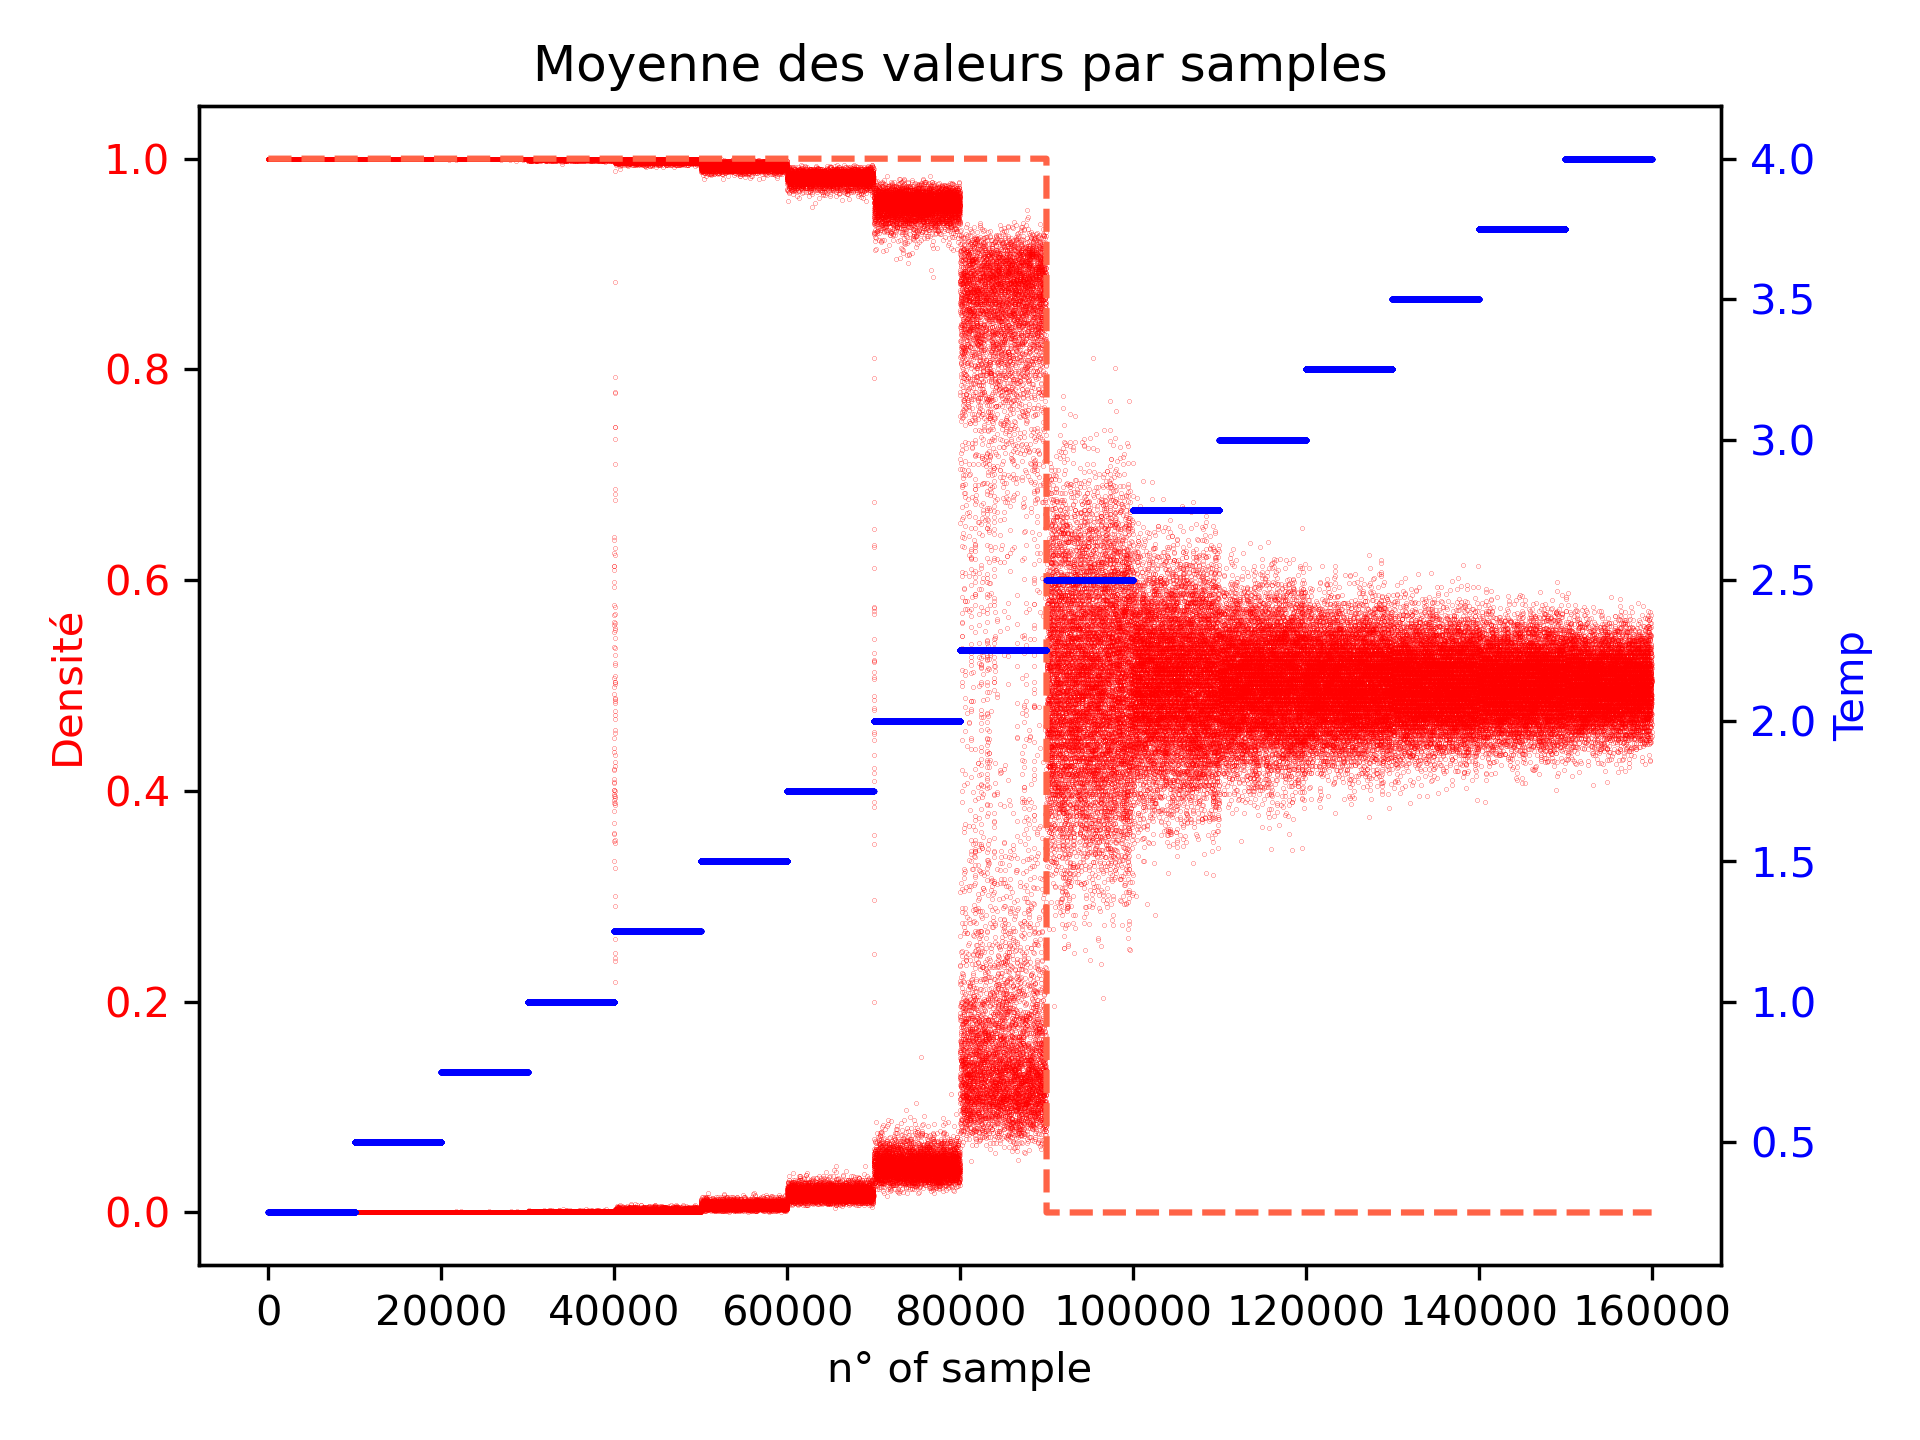
\includegraphics[width=0.95\linewidth]{./figures/raw_data.png}
		\caption{Données brutes}
		\label{fig:rawdata}
	\end{subfigure}
	\begin{subfigure}{0.5\textwidth}
		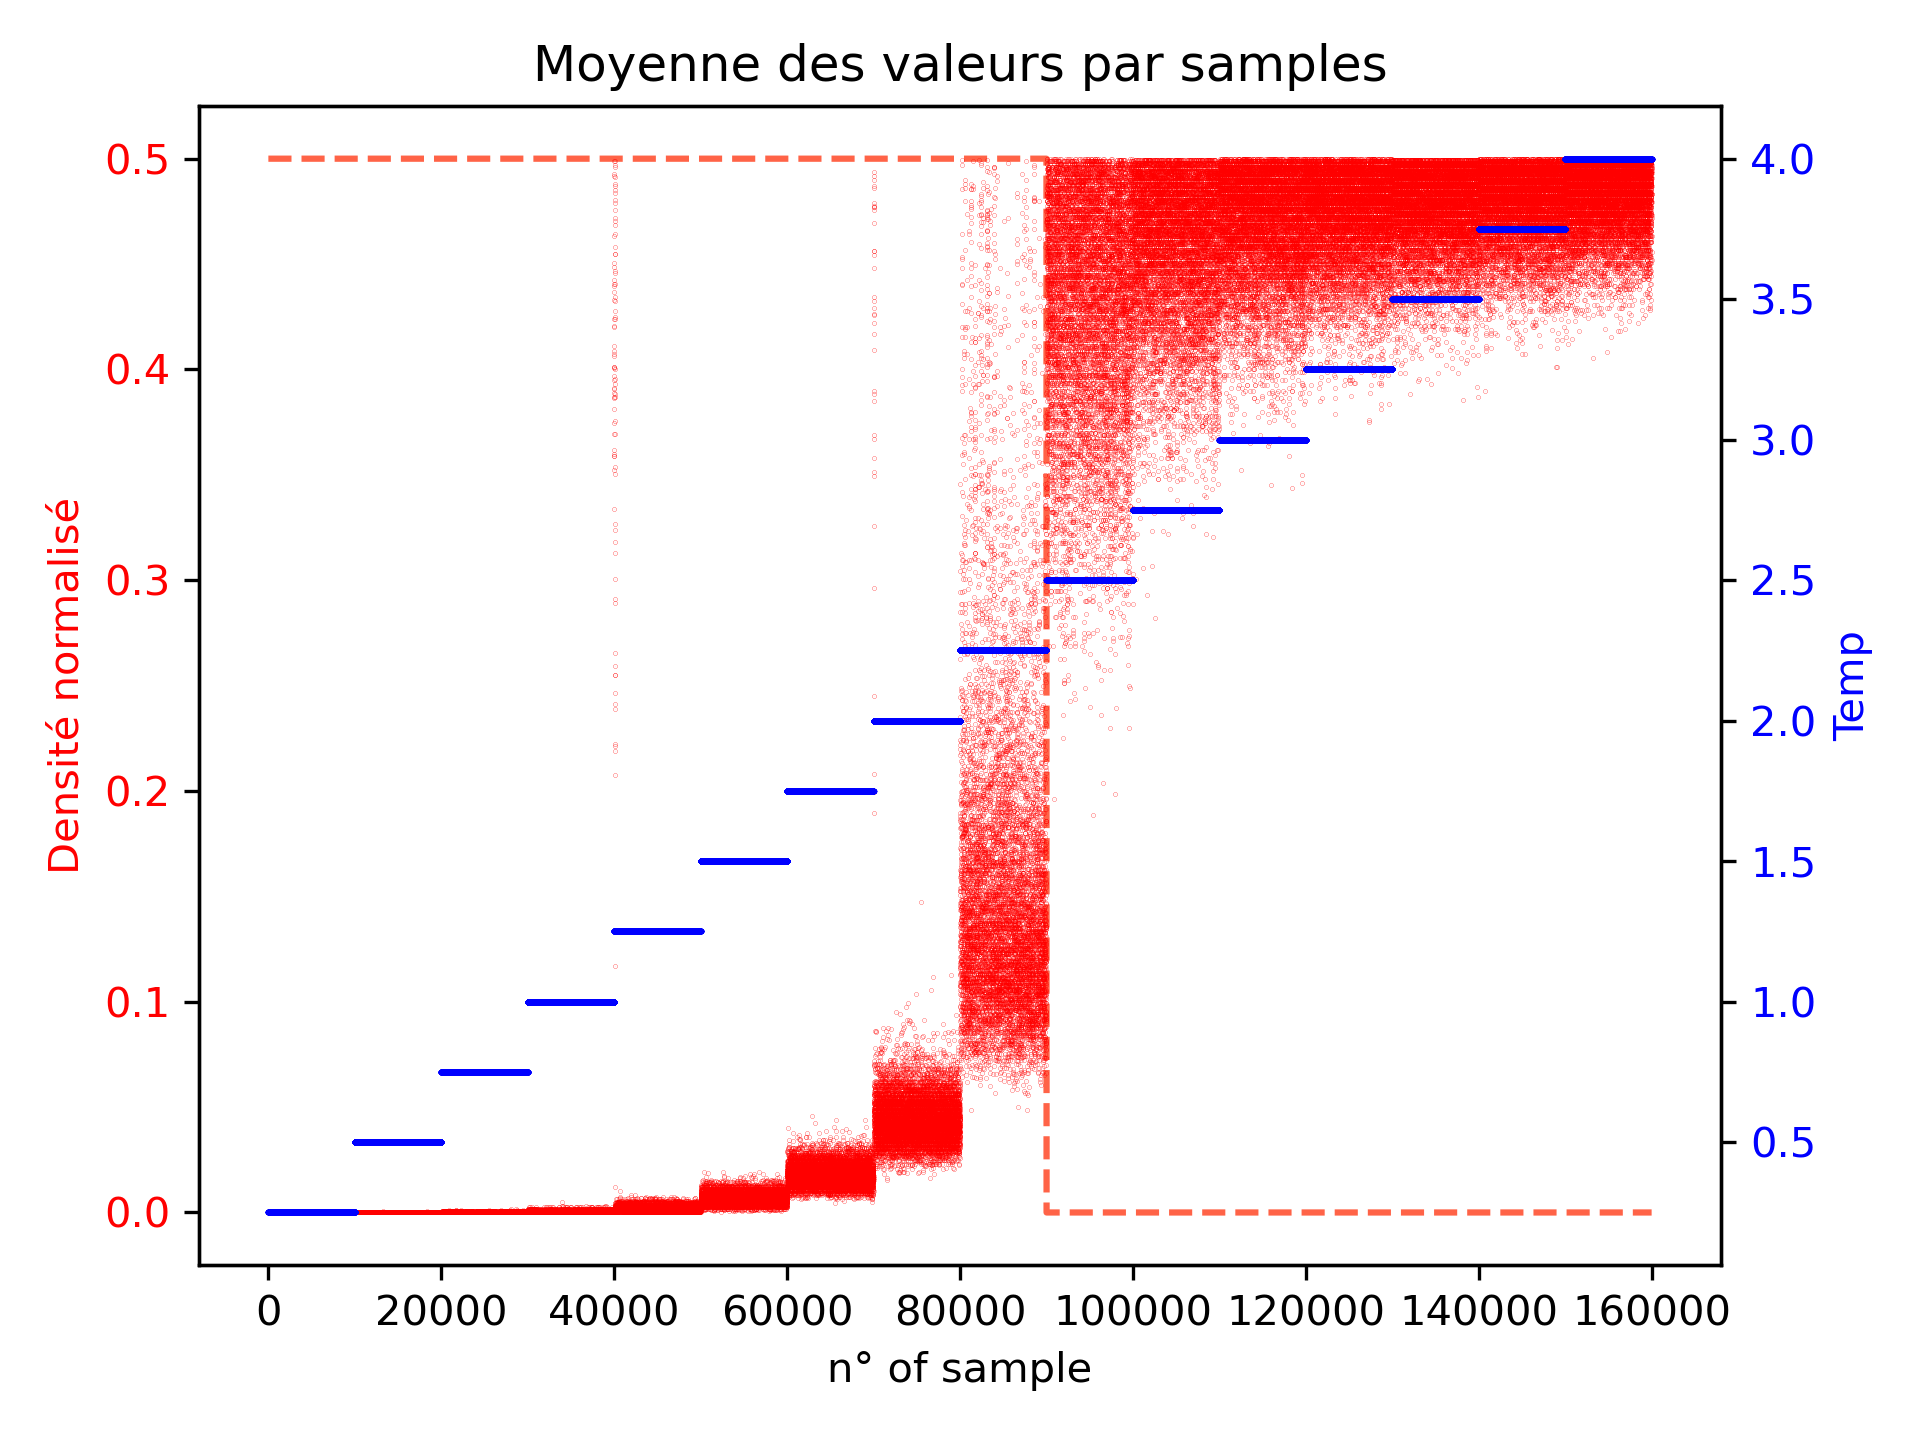
\includegraphics[width=0.95\linewidth]{./figures/sym_data.png}
		\caption{Données symétrisées}
		\label{fig:symdata}
	\end{subfigure}
	\caption{}
\end{figure}

Dans la partie suivante, nous allons entraîner certains modèles spécifiques sur la densité de spin symétrisée. Dans ce cas, nous allons aussi normaliser afin de rendre les modèles plus performants.
Pour cela, nous allons utiliser la méthode \textit{StandardScaler} de la librairie \textit{sklearn} qui permet de centrer et réduire les données. Cette méthode soustrait la moyenne et divise par l'écart-type. Ainsi, on se retrouve avec des données centrées en $0$ et de variance $1$.

Il nous faut maintenant séparer nos données en deux ensembles : un ensemble d'entraînement et un ensemble de test. Pour cela, nous allons utiliser la méthode \textit{train\_test\_split} de la librairie \textit{sklearn}. Cette fonction nous permet de préciser le taux de répartition des données entre l'ensemble d'entraînement et l'ensemble de test. Nous allons répartir $80\%$ des données dans l'ensemble d'entraînement et $20\%$ dans l'ensemble de test. De plus, cela nous permet de mélanger les données avant de les répartir afin d'avoir dans les deux ensembles des données représentatives de notre jeu de données originel.

Afin d'appliquer exactement la même transformation sur les données de test, nous allons créer un pipeline qui va appliquer la méthode de symétrisation puis la méthode de normalisation. Ainsi, on pourra appliquer le pipeline sur les données de test sans avoir à les modifier.
Finalement, certains modèles seront plus réceptifs à des données présentées sous forme de vecteur de taille $1600$, d'autre sous forme de matrice de taille $40 \times 40$. Pour éviter de devoir modifier les données à chaque fois, nous allons créer un pipeline qui va transformer les données en matrice si nécessaire et appliquer les autres méthodes de pré-traitement expliquées ci-dessus.

\newpage
\section{Modèles classiques}

\subsection{Analyse par la magnétisation}
Notre première approche de ce problème est de considérer la magnétisation comme une fonction de la température. Cette approche nous permet de réduire grandement la complexité du problème. En effet, nous n'avons plus qu'une seule variable à considérer : l'état moyen des spins. Dans cette partie, nous allons donc essayer de prédire la température à partir de la magnétisation. Il suffit ensuite de comparer la valeur prédite à la valeur de la température critique pour déterminer la phase du système.

Avant tout, nous allons établir un modèle naïf qui va nous servir de référence. Ce modèle va simplement renvoyer la valeur moyenne de la température du jeu de données. Ainsi, on pourra comparer les performances de nos modèles avec ce modèle naïf. On obtient une erreur quadratique moyenne de $1.32$.

Du fait du bruit de nos données et du faible nombre de températures distinctes, nous devons porter une attention particulière au sur-apprentissage de nos modèles.
Prenant en compte le grand nombre de données, nous sommes partis sur un modèle de foret aléatoire. Ce modèle est très robuste et permet de limiter le sur-apprentissage. De plus, il est très rapide à entraîner et à tester.
Au niveau des hyperparamètres, nous avons limité la profondeur des arbres à 5 et nous avons aussi composé la foret de $100$ arbres. De plus, la méthode de \textit{Bootsrap} est activée. Cette méthode permet de créer des sous-ensembles de données de la taille de l'ensemble de données originale. Ainsi, on peut entraîner plusieurs arbres sur des données différentes et les combiner pour obtenir un modèle plus robuste.
On peut donc limiter le sur-apprentissage tout en gardant un modèle performant. Les résultats obtenus sont présentés sur la figure \ref{fig:forest}.
La figure \ref{fig:forest} possède deux objets : La densité de points de la moyenne des spins symétrisée par température calculée en utilisant la méthode de \textit{KDE} (\textit{Kernel density estimation}) et la prédiction du modèle de fôret aléatoire.

Avec une MSE de $0.108$, on obtient un modèle qui est $12$ fois plus performant que le modèle naïf. Cependant, on peut voir que le modèle a du mal à distinguer les hautes températures. En effet, les valeurs prédites par ce modèle sont toujours inférieures à $3.5$.
Cela peut s'expliquer par le fait que, à haute température, la densité est quasiment nulle. Ainsi, lorsque le modèle va essayer de prédire une configuration de spin à haute température, il va prédire la température correspondant plus ou moins à la moyenne des températures capables de produire une configuration de spin similaire. Cela apparaît clairement sur la figure \ref{fig:forest}.

Nous pouvons, maintemant, utiliser la prédiction en température de notre modèle pour déterminer la phase du système. Pour cela, nous allons comparer la valeur prédite à la valeur de la température critique. Si la valeur prédite est supérieure à la valeur de la température critique, alors le système est dans la phase paramagnétique. Sinon, il est dans la phase ferromagnétique.
Théoriquement, la température critique d'un modèle d'Ising 2D est de $2.269$ \cite{aviles_critical_2023}. On retrouve les résultats de cette analyse sur la figure \ref{fig:forest_matrix}.  Notre modèle est capable de prédire la phase du système avec une précision de $98.8\%$. On a donc un modèle performant.

\begin{figure}[h]
	\begin{subfigure}[c]{0.65\textwidth}
		\centering
		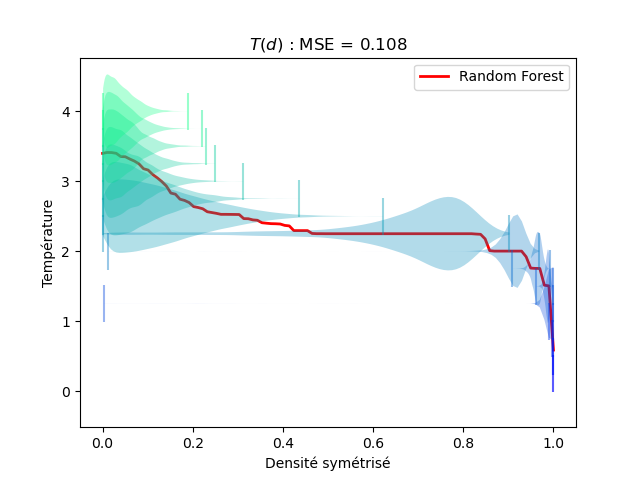
\includegraphics[width=1.1\linewidth]{./figures/forest.png}
		\caption{Résultats du modèle}
		\label{fig:forest}
	\end{subfigure}
	\begin{subfigure}[c]{0.3\textwidth}
		\centering
		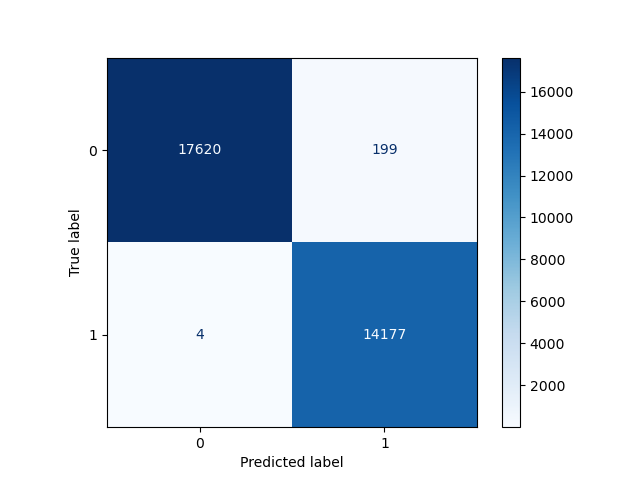
\includegraphics[width=1.3\linewidth]{./figures/forest_matrix.png}
		\caption{Matrice de confusion}
		\label{fig:forest_matrix}
	\end{subfigure}
	\caption{Modèle de foret aléatoire}
\end{figure}

\subsection{Analyse par l'état individuel des spins}
Dans cette partie, notre objectif était de développer des modèles naïfs afin d’obtenir des scores de référence, pour ensuite avoir une référence de la performance et évaluer la robustesse de notre modèle performant. Pour cela, nous avons décidé de créer un modèle basé sur le hasard, puisque qu’on a jugé que c’était le modèle moins efficace. Nous allons maintenant analyser ce modèle et évaluer ces performances. 

On part du principe que sans modèle, on aurait une chance de 50\% de prédire la transition de phase. Cela est dû au fait que nous pouvons simplifier cette approche par le concept que la donnée considérée est soit en transition de phase ou elle ne l’est pas. Notre modèle basé sur le hasard suit ce concept. Cependant, ce modèle est toujours un peu bruité, dû au fait que les proportions de données appartenant à la classe positive ne correspondent pas à celles de classe négative.

Analysons maintenant les performances de ce modèle. Pour ce modèle, on trouve une MSE (\textit{Mean Squared Error}) $= 0.49$. Cela indique que les prédictions du modèle sont considérablement éloignées des vraies valeurs. Ce modèle n’est pas capable de capturer efficacement les caractéristiques nécessaires à la transition de phase. Pour la précision, on obtient une valeur de $0.51$, soit presque la moitié correctement classée, proche de la valeur attendue de 50\%. On confirme alors que le modèle n’a pas réussi à surpasser l’approche aléatoire. 

Finalement, nous avons réalisé la matrice de confusion, que nous observons à la figure \ref{fig:random_matrix}. Cette matrice révèle davantage les performances du modèle. Les résultats indiquent que le modèle prédit correctement 51\% des échantillons. Cela nous montre à nouveau l’inefficacité du modèle à distinguer les deux classes. 

Le modèle basé sur le hasard ne réussit pas à faire des prédictions significatives pour cette tâche de classification binaire. Ces évaluations de la performance de ce modèle que nous avons fait montrent bien ces limites et donc il est nécessaire de réaliser un modèle plus complexe.

\begin{figure}[h]
	\centering
	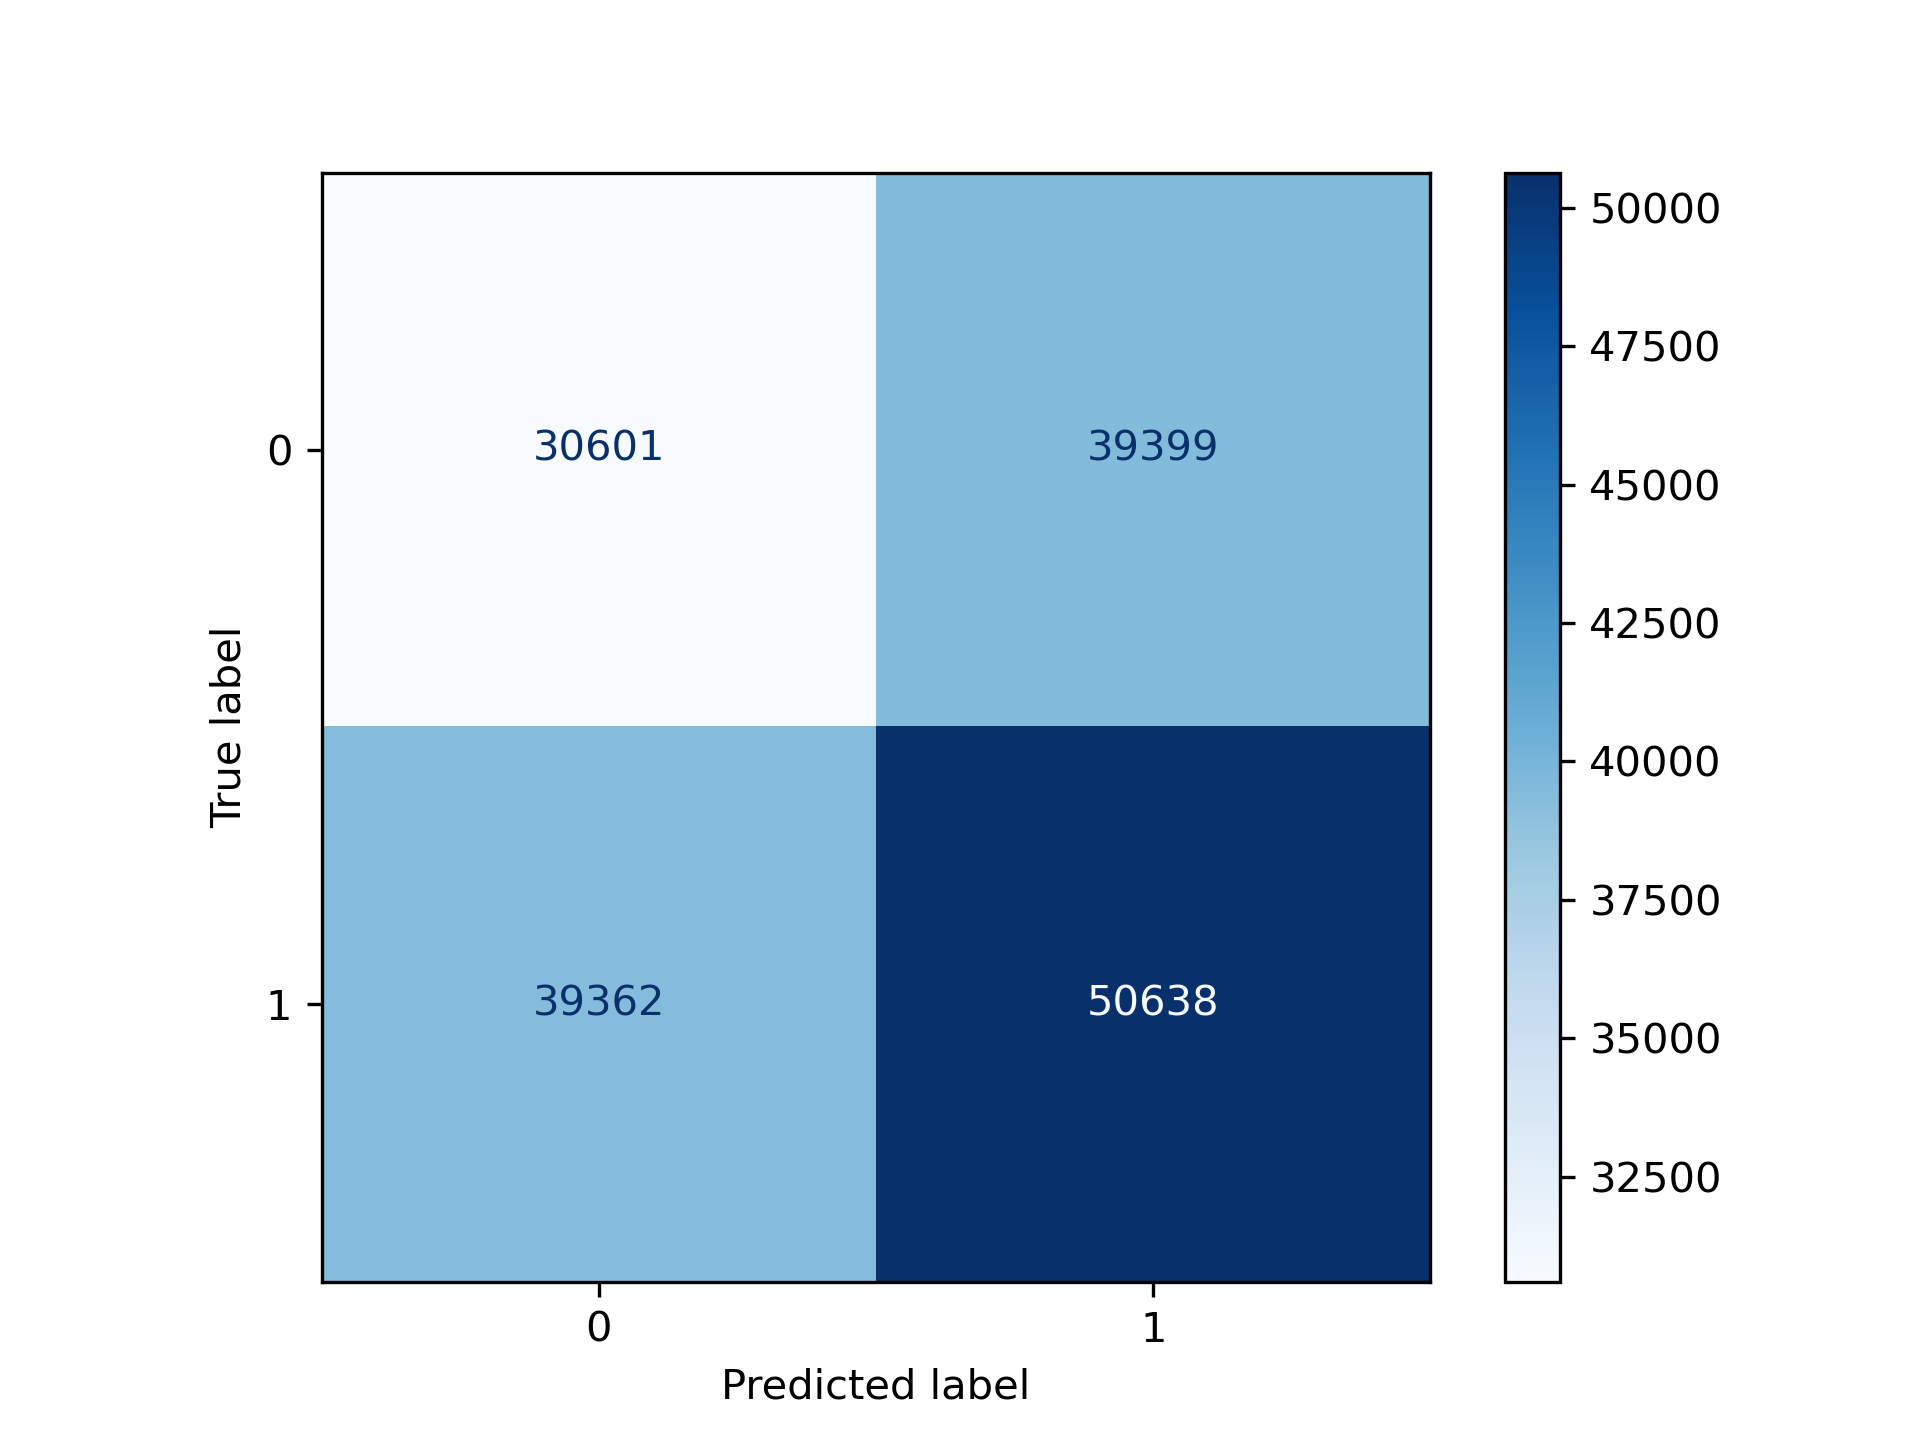
\includegraphics[width=0.44\linewidth]{./figures/random_matrix.png}
	\caption{Matrice de confusion du modèle basé sur le hasard}
	\label{fig:random_matrix}
\end{figure}

\newpage
\section{Réseaux de neurones}
\subsection{Objectif}
Dans le cadre de ce projet, notre objectif final était de développer un modèle performant capable de classer des matrices de taille 40x40 en deux catégories distinctes. Comme dans le modèle d’Ising l’état d’un spin est dépendant de ces plus proches voisins, le plus naturel était de créer un réseau neuronal convolutif car il prend en compte les corrélations locales entre pixels voisins. La performance de notre classification est alors dépendante de l’architecture de notre modèle, de la manière dont il extrait et apprend les caractéristiques pertinentes des matrices en entrée.

Dans cette partie, nous allons analyser l’architecture du modèle qu’on a créé. On va discuter pourquoi on a choisi chaque couche et quel rôle elles jouent dans notre modèle. On analysera ensuite nos étapes d’entraînement puis on discutera les méthodes que nous avons utilisées pour évaluer nos performances.

\subsection{Architecture du modèle}
L’ensemble de l’architecture repose sur des principes de convolution, pooling et de couches entièrement connectées. La combinaison de ces différentes couches crée une architecture cohérente et un modèle performant.

Notre modèle commence par une première couche de convolution 2D, qui utilise 16 filtres de taille 5x5. Cette couche veut extraire des caractéristiques de bas-niveau, soit des bords ou des formes simples présentes dans les données. Cette première couche de convolution est suivie d’une couche de max pooling qui permet, en faisant un sous-échantillonnage, de compresser l’information que l’on veut faire passer à la couche suivante.

On applique ensuite à nouveau ce processus : on a une deuxième couche de convolution 2D à 32 filtres de taille 3x3 et une nouvelle couche de max pooling. Avec cette deuxième couche de convolution, on souhaite capturer des motifs plus complexes et abstraits. On a augmenté le nombre de filtres de la première couche de convolution car on veut augmenter la capacité du modèle : chaque filtre pourra se spécialiser dans la détection de certaines caractéristiques et donc le modèle apprendra plus de relations complexes. Avec la couche de max pooling, on souhaite réduire davantage la dimension spatiale. Finalement, on utilise une dernière couche de convolution 2D avec 64 filtres de taille 3x3, suivie encore d’une autre opération de max pooling.

Ensuite, on utilise une couche Flatten pour aplatir les caractéristiques et motifs extraits de nos couches de convolution pour réduire la dimension de notre matrice. Il s’agit d’une opération assez simple avant d’introduire des couches entièrement connectées Dense. On a utilisé trois couches consécutives : la première avec 128 neurones, la deuxième avec 64 neurones puis la troisième avec 128 neurones. Ces trois couches ont comme objectif d’apprendre les complexités des caractéristiques extraites, afin de réaliser l’objectif de notre modèle. Notre deuxième couche Dense a moins de neurones pour réduire les dimensions et additionner encore un peu de complexité à notre modèle, afin de tout bien représenter. Cette architecture que nous avons utilisée permet une certaine flexibilité au modèle et de s’adapter à la tâche de la classification binaire.

Finalement, l’architecture de notre modèle se termine par une couche de sortie avec une seule cellule, activée à la fonction d’activation sigmoïde. Cela nous permet d’obtenir à la sortie de notre modèle une probabilité que notre sortie appartienne à la classe positive, ce qui correspond bien à ce qui est attendu lors d’une classification binaire.

L’architecture de notre modèle est présentée sous forme d’image dans la figure \ref{fig:model}

\subsection{Entraînement du modèle}
La procédure d’entraînement consiste à entraîner le modèle à réaliser une classification binaire : identifier s’il y a eu une transition de phase par rapport aux matrices qui décrivent notre système. Avant l’entraînement, nous avons compilé notre modèle avec l’algorithme optimiseur Adam et on a utilisé binary crossentropy comme fonction de coût, une fonction de coût très efficace pour les tâches de classification binaire qui mesure la différence entre les prédictions binaires et les vrais résultats. Finalement, l’entraînement de notre modèle a duré que 11 epochs, avec un batch size de 128. Notre entraînement a duré que 11 epochs pour éviter le sur-apprentissage, puisque nous avons utilisé la méthode de l’arrêt anticipé (early stopping), avec une patience de 5. L’entraînement du modèle a été fait avec les $160 \ 000$ matrices que l'on nous a fournies et a pris que 40 secondes.

Pendant l’entraînement, l’erreur d’entraînement et l’erreur de validation sont enregistrés pour chaque epoch. Cela nous permet de suivre l’entraînement de notre modèle et de détecter des signes de sur-apprentissage ou sous-apprentissage. En suivant cette approche et cette architecture, nous sommes parvenus à un modèle très efficace, dont nous allons étudier les performances maintenant.

\subsection{Evaluation des performances du modèle}
L’objectif principal du modèle est de capturer des motifs complexes qui permettront au modèle d’apprendre les complexités de nos matrices données en entrée et puis faire des prédictions sur à quelle classe appartient chaque matrice. Avec l’enregistrement de l’entraînement et la possibilité de faire des essais avec notre jeu de test, on peut évaluer notre modèle.

Tout d’abord, on peut analyser la performance de notre modèle en prenant en compte la même métrique qu'utilisé sur les autres modèles. On applique donc la \textit{mse} sur l’ensemble de données de validation, qui est de seulement $1.37\times 10^{-3}$. Cette valeur est près de $350$ fois plus faible que la classification naïve. Cela indique que le modèle est très performant : il a atteint un niveau très bas de perte sur les données de validation et a une très bonne capacité de se généraliser à de nouvelles données. On peut aussi vérifier la précision (accuracy) de notre modèle sur les données de test : 0.99. Notre modèle est capable de classer correctement 99\% des échantillons dans l’ensemble de test. Cela renforce à nouveau l’idée que notre modèle a une très bonne capacité à généraliser et qu’il est très adéquat à la classification binaire. Nous avons aussi calculé une autre métrique intéressante : la sensibilité, mesurant la capacité du modèle à identifier tous les exemples positifs réels dans l'ensemble de données et nous trouvons une valeur de 0.99, indiquant une excellente capacité à mesurer des vrais positifs.

Ensuite, nous pouvons étudier l’entraînement de notre modèle. Dans la figure \ref{fig:train}, nous observons l’évolution de l’erreur de la fonction de coût des données d’entraînement et de validation au cours de l’entraînement (graphe en haut). On remarque que les courbes représentant ces données sont très proches dès la première epoch jusqu’à l’epoch 6 et puis commencent à diverger ce qui peut être un signe de sur-apprentissage. Cependant, cela peut être négligeable dû à la simple différence de 0.005 entre les deux courbes. On souligne encore que l’évolution de l’entraînement est très légère, sans grande amélioration de l’erreur sur la fonction de coût. Encore dans la figure \ref{fig:train}, on observe l’évolution de la précision au cours de l’entraînement (graphe en bas). On remarque que dès la première epoch jusqu’à la fin de l’entraînement, ces deux courbes sont toujours très proches autour de 0.998, ce qui confirme à nouveau excellente précision de notre modèle.

\begin{figure}[h]
	\centering
	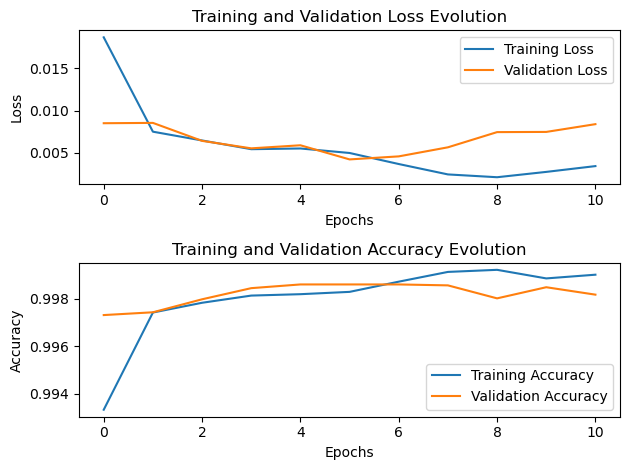
\includegraphics[width=0.66\linewidth]{./figures/train.png}
	\caption{Évolution de l'entraînement}
	\label{fig:train}
\end{figure}

De plus, nous pouvons établir la matrice de confusion de notre modèle, que nous pouvons observer à la figure \ref{fig:matrix_CNN}. La matrice de confusion résume le nombre de prédictions correctes et incorrectes faites par le modèle sur l’ensemble des données de test. On observe les vrais négatifs et les vrais positifs, représentés respectivement en haut à gauche et en bas à droite de la matrice de confusion. Ces nombres représentent les prédictions correctes du modèle, où il a réussi à identifier correctement les instances des deux classes,  c’est-à-dire s’il y avait une transition de phase ou pas. Lors des prédictions sur le jeu de test, nous avons 14 158 vrais négatifs (nombre d’échantillons qui étaient réellement dans la classe 0 et correctement identifiés par le modèle) et 17 781 vrais positifs (classe 1 correctement identifiée). De plus, on peut encore observer les faux négatifs et les faux positifs, représentés respectivement en bas à gauche et en haut à droite de la matrice de confusion. Ils représentent les erreurs de classification du modèle. On a 36 faux négatifs et 23 faux positifs, ce qui est négligeable face au nombre de prédictions correctes. Le modèle créé est alors extrêmement efficace à prédire la transition de phase.

\begin{figure}[h]
	\begin{subfigure}[c]{0.5\textwidth}
		\centering
		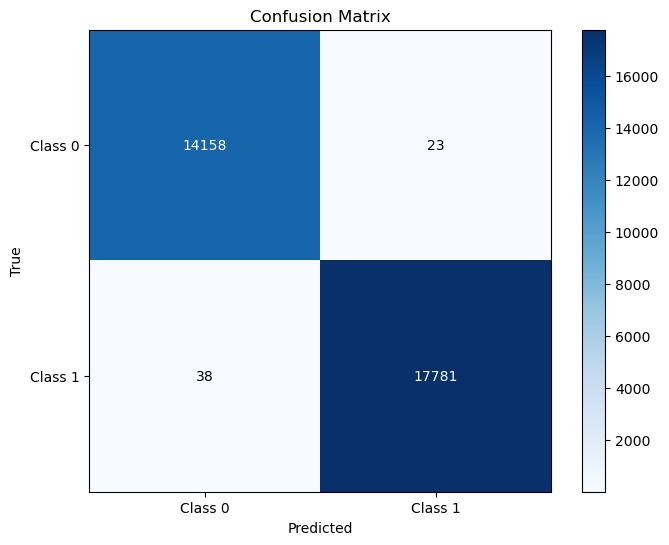
\includegraphics[width=0.9\linewidth]{./figures/matrix_CNN.png}
		\caption{Matrice de confusion}
		\label{fig:matrix_CNN}
	\end{subfigure}
	\begin{subfigure}[c]{0.5\textwidth}
		\centering
		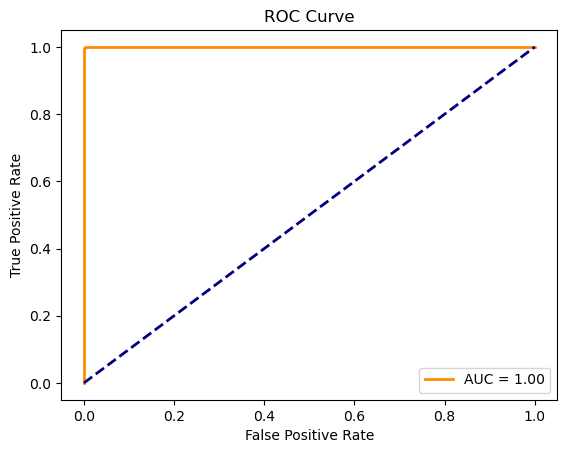
\includegraphics[width=0.9\linewidth]{./figures/ROC.png}
		\caption{Courbe ROC}
		\label{fig:ROC}
	\end{subfigure}

\end{figure}

Finalement, nous pouvons tracer la courbe ROC (Receiver Operating Characteristic), vue dans la figure \ref{fig:ROC}. Il s’agit d’un autre outil d’évaluation de la performance d’un modèle de classification binaire. Elle représente graphiquement la relation entre le taux de vrais positifs, connu aussi comme la sensibilité (ou recall) et le taux de faux positifs lorsqu’on fait varier le seuil de classification. On observe qu’on obtient un AUC (Area Under Curve) de 1.00, ce qui nous indique une performance exceptionnelle de notre modèle. Une valeur de 1.00 signifie une séparation parfaite des classes. Le modèle est très précis dans sa capacité à distinguer les exemples positifs des négatifs.

\begin{figure}[h]

\end{figure}

Dans cette partie, nous avons construit un réseau neuronal convolutif performant capable de classer efficacement nos données par rapport à l’existence ou pas d’une transition de phase. L’architecture du modèle choisi permet d’extraire les caractéristiques complexes de nos données et l’entraînement a été optimisé pour cette tâche de classification binaire. Les métriques de notre modèle, telles que la précision, la sensibilité, la matrice de confusion et la courbe ROC montrent la robustesse de notre modèle. Nous avons alors créé un modèle à la fois précis et efficace, qui démontre une performance exceptionnelle dans le classement des matrices du modèle Ising.

\newpage
\section{Génération d'images}
Dans cette partie, nous allons étudier comment générer de nouvelles images crédibles à partir du jeu de données à l'aide de réseaux convolutionnels.

Cette section reste inachevée en raison des difficultés rencontrées lors de la génération de ces modèles. En tant qu'auteur de tous ces réseaux (environ 300 essais avec différentes architectures), je pense que le problème réside dans la nature des images. Ce sont des images de bruit. Au-delà de la température de Curie, les images se ressemblent toutes, peu importe la température. Il est donc difficile pour l'ordinateur de comprendre quelle image est associée à quelle température, ce qui est également le cas pour les basses énergies.

Un deuxième problème est que les réseaux convolutionnels ont tendance à créer des images bruitées ou floues, ce qui n'aide pas l'algorithme à produire des images nettes de bruit composées strictement de 0 et de 1, même avec des fonctions d'activation sigmoid à la fin du parcours.

\subsection{Auto-encodeur}
Nous allons discuter de l'une des méthodes que nous avons choisies pour générer de nouvelles données. La technique des autoencodeurs est une approche de synthèse d'image basée sur l'utilisation de deux sous-réseaux de neurones mis bout à bout. Le premier, l'encodeur, est un réseau qui prend en entrée une image et, par réduction de dimension successive, parvient à un sous-espace de dimension inférieure appelé "espace latent". Cet espace latent est censé concentrer l'information de l'image dans un format plus compact. La deuxième partie de l'autoencodeur est le décodeur, un réseau qui part de l'espace latent et augmente ses dimensions jusqu'à atteindre la dimension souhaitée, qui est celle d'une nouvelle image.

Le réseau s'entraîne en partant d'une image du jeu de données d'entraînement, puis, cherche à reproduire une image du même ensemble de données. Il peut s'agir de la même image ou d'une autre, l'objectif étant de générer une nouvelle image cohérente.

L'entraînement de l'encodeur et du décodeur se déroule de manière intégrée, les deux réseaux formant ainsi un seul réseau. Une fois que l'autoencodeur est entraîné, il peut être dissocié. On peut alors utiliser l'encodeur pour réduire dans l'espace latent toutes les images du jeu d'entraînement ou du jeu de test associées à une température donnée. Cela permet de générer dans l'espace latent le vecteur caractéristique de la température spécifiée. Ce vecteur caractéristique représente en réalité une direction dans un espace de dimension définie par l'espace latent, associée à une caractéristique dominante du jeu de données d'entraînement. Ainsi, il est possible de créer un nouveau vecteur pointant dans cette direction pour générer, à l'aide du décodeur, de nouvelles images.

\begin{figure}[h]
	\centering
	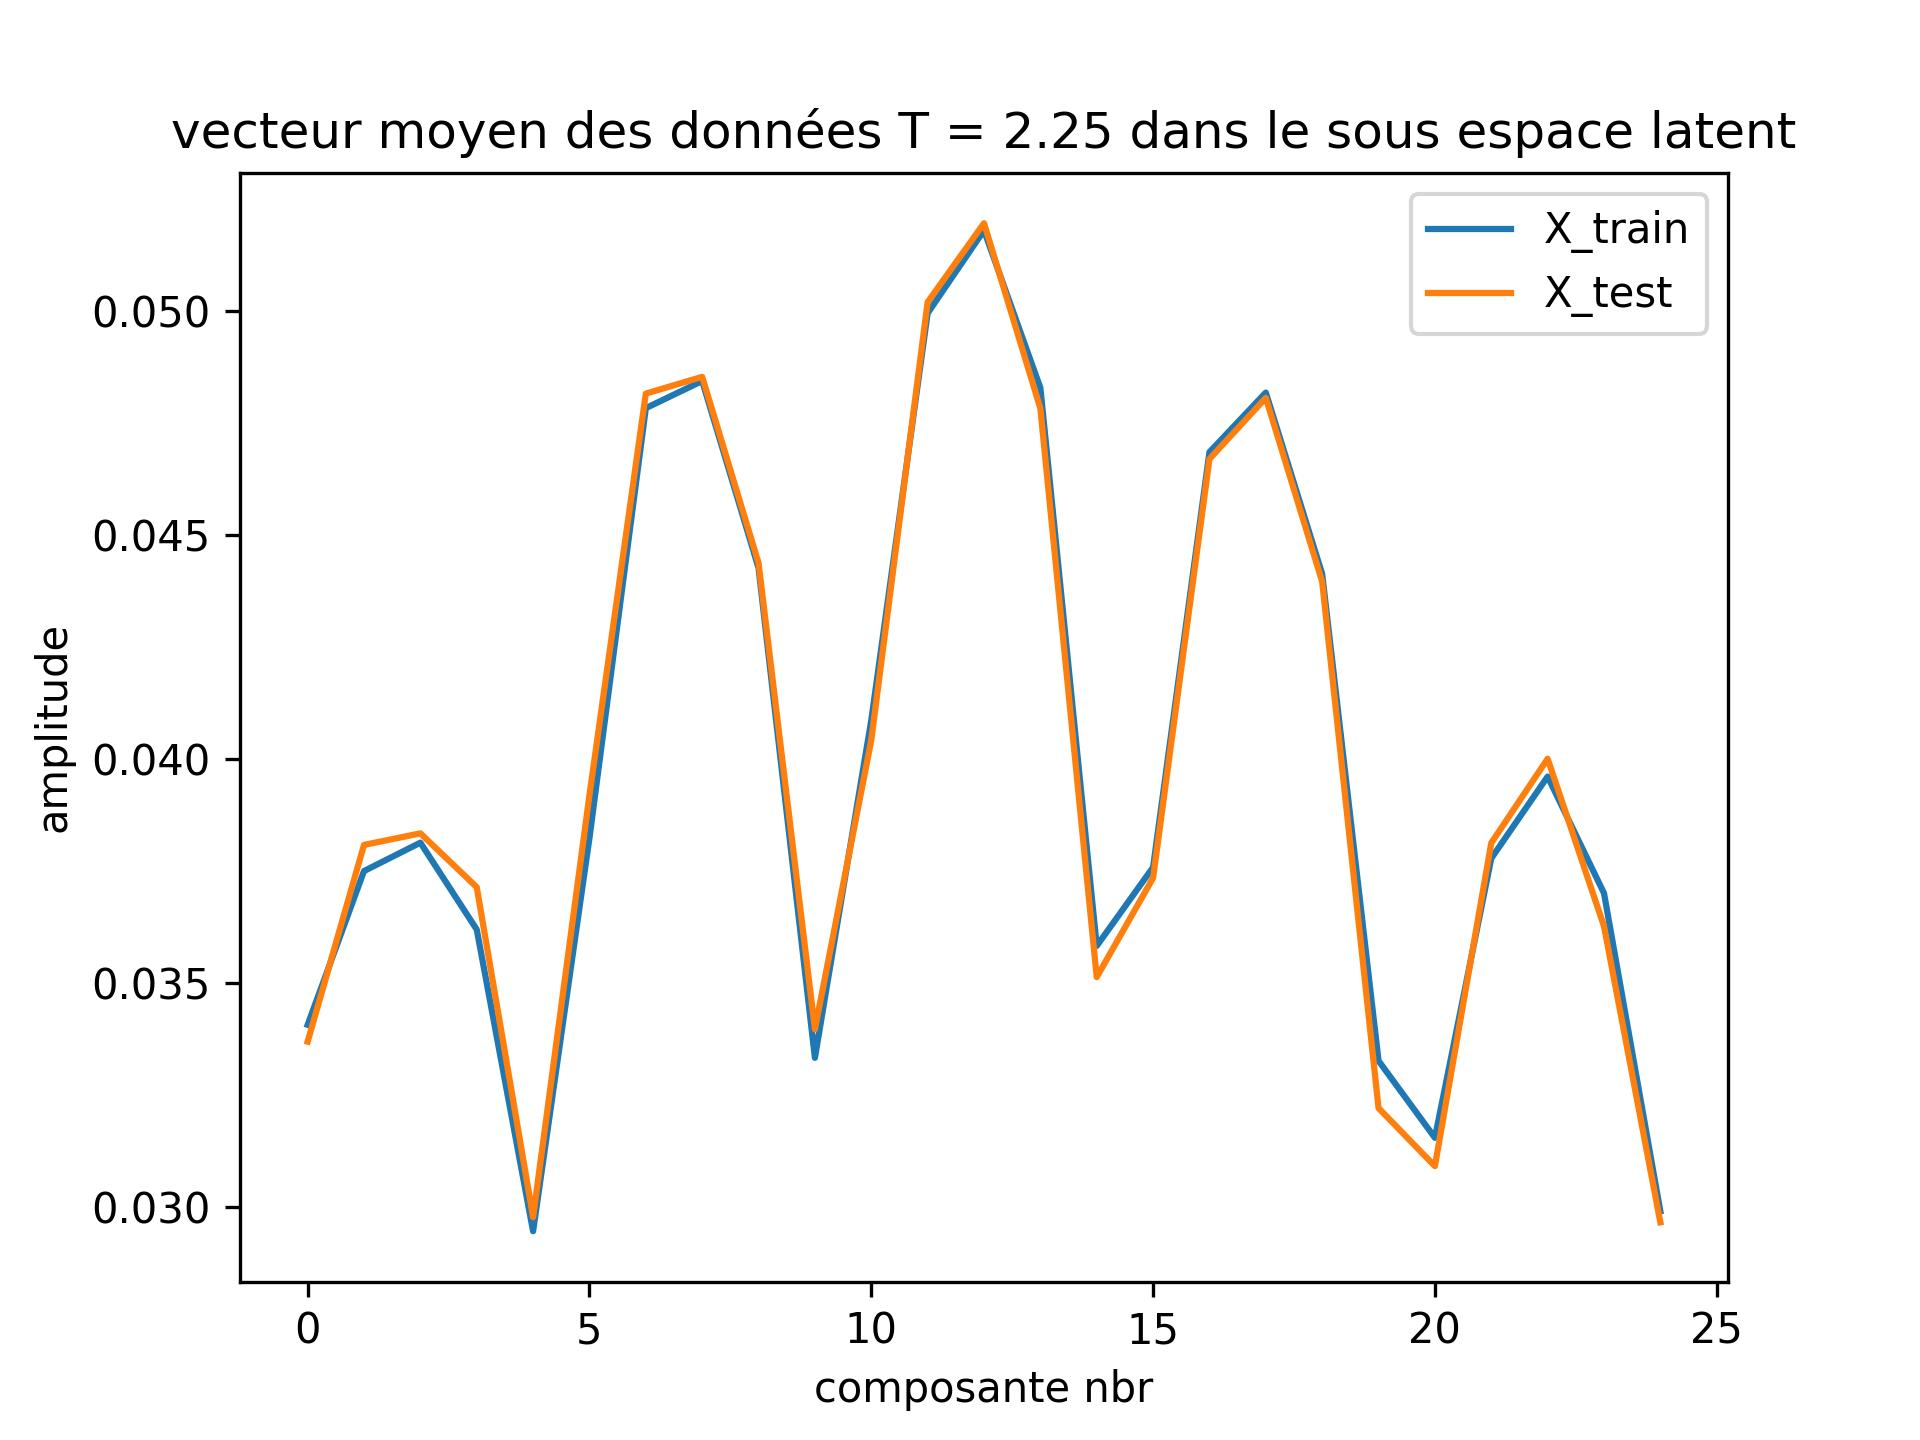
\includegraphics[width=0.5\linewidth]{./figures/latent.jpg}
	\caption{Représentation dans l'espace latent}
	\label{fig:latent}
\end{figure}

Cette reconstruction est souvent sujette à une certaine imprécision, nécessitant ainsi l'ajout d'un traitement postérieur pour assurer la cohérence de l'image de sortie (cf. figure \ref{fig:tiple}). J'applique un seuillage ainsi que l'ajout de bruit pour faire ressortir des zones sombres avec un soupçon de blanc, et des zones blanches avec une touche de sombre. Il s'agit d'un traitement encore à un stade prototypique.

L'entraînement se révèle capricieux lorsque la température (T) est élevée, mais devient plus stable à basse température, ce qui est normal étant donné que tous les filtres convergent vers 0.

\begin{figure}[h]
	\begin{subfigure}[c]{0.5\textwidth}
		
		\centering
		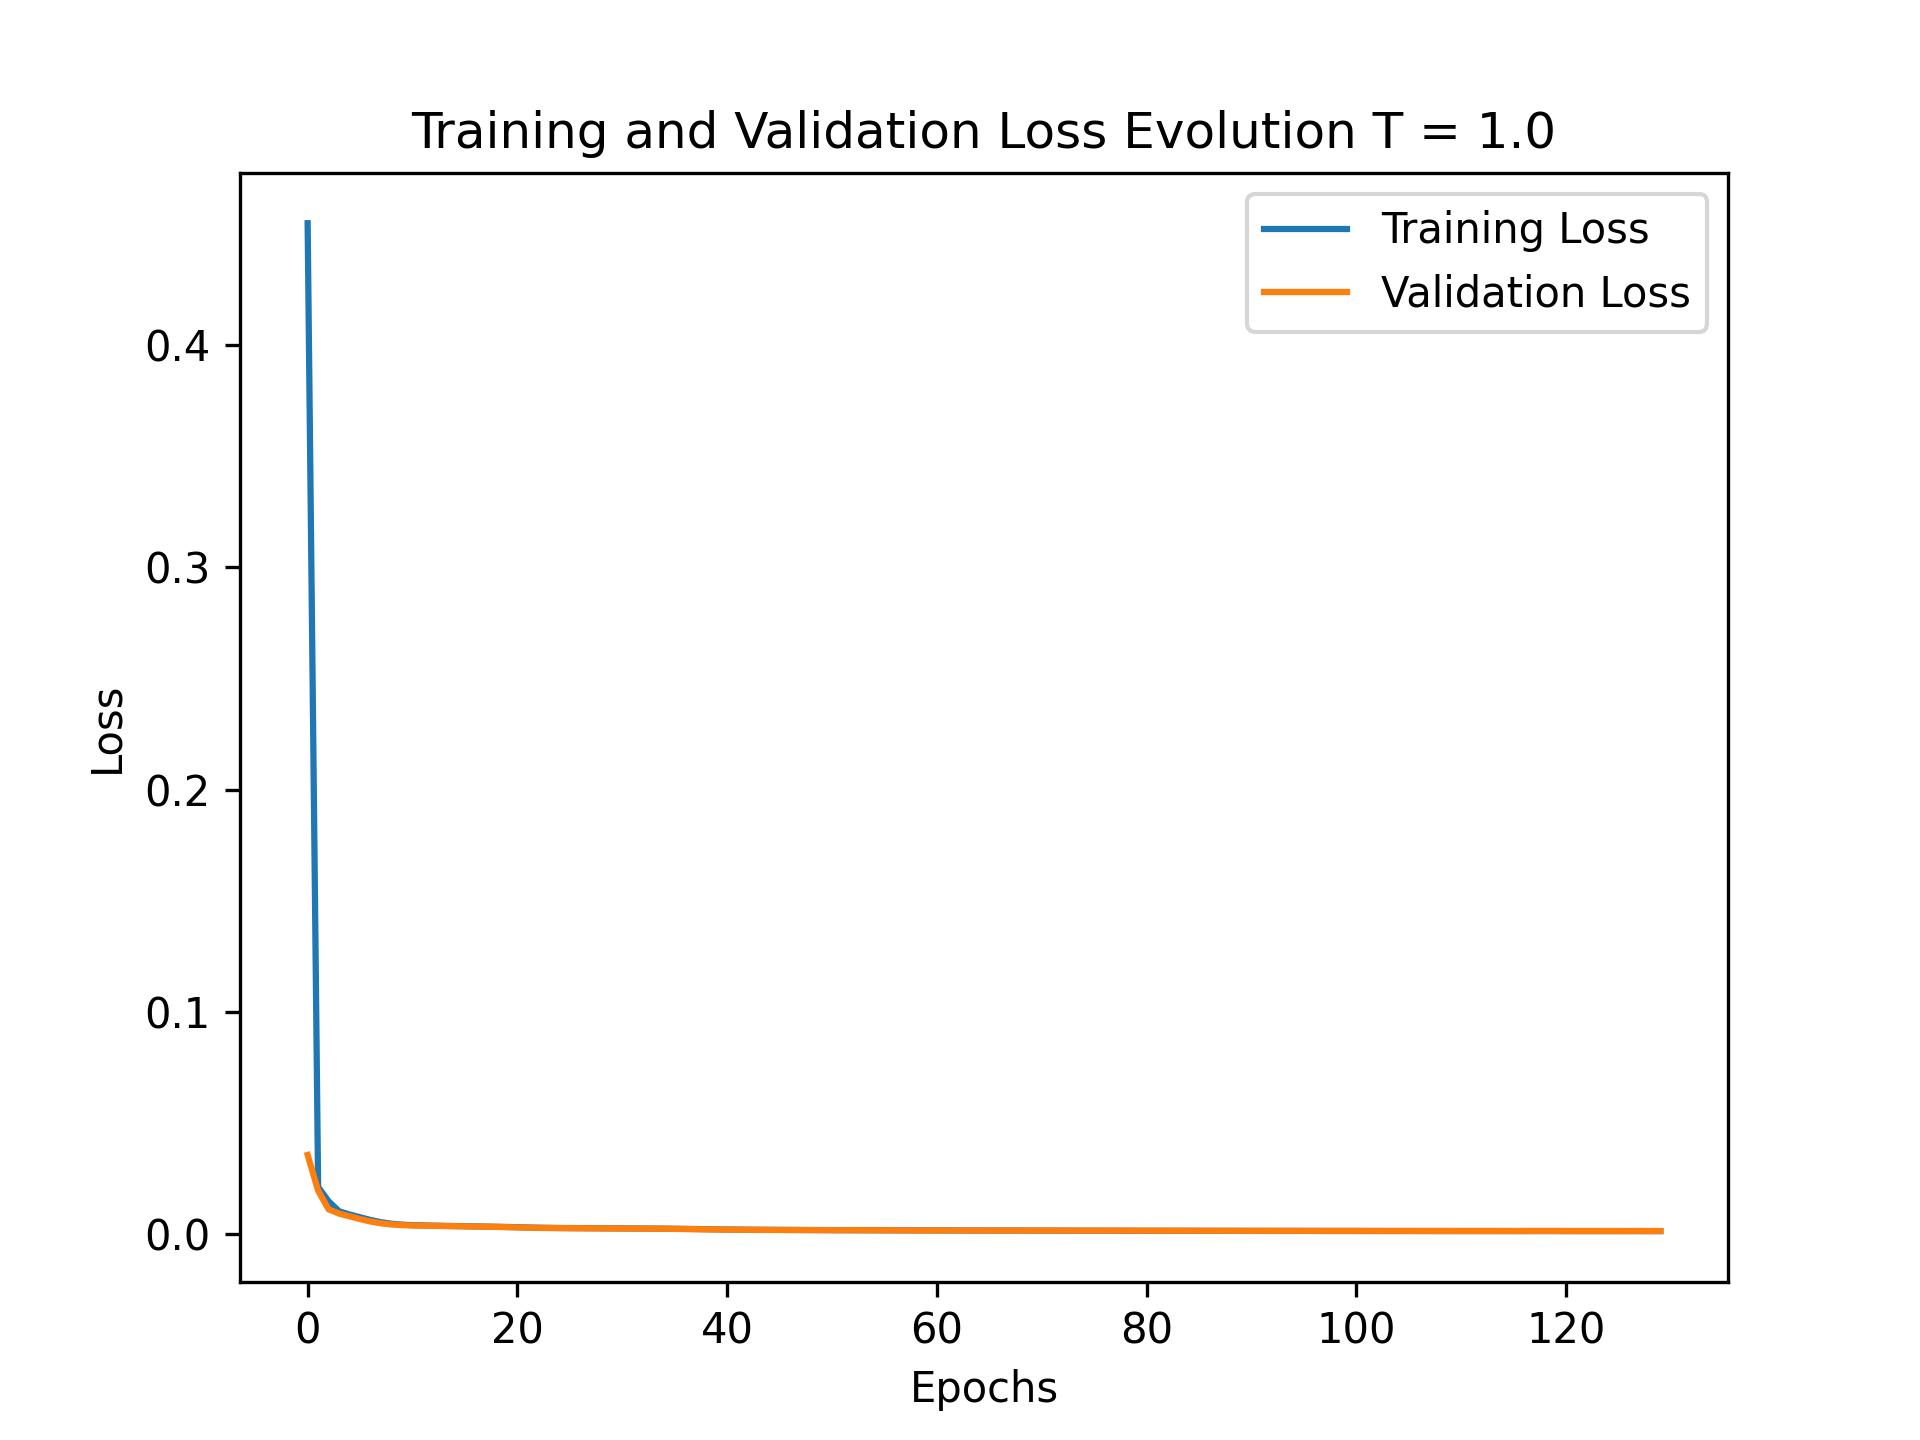
\includegraphics[width=0.9\linewidth]{./figures/evol_T_1.jpg}
		\caption{$T = 1.00$}
		\label{fig:T1}
	\end{subfigure}
	\begin{subfigure}[c]{0.5\textwidth}
		\centering
		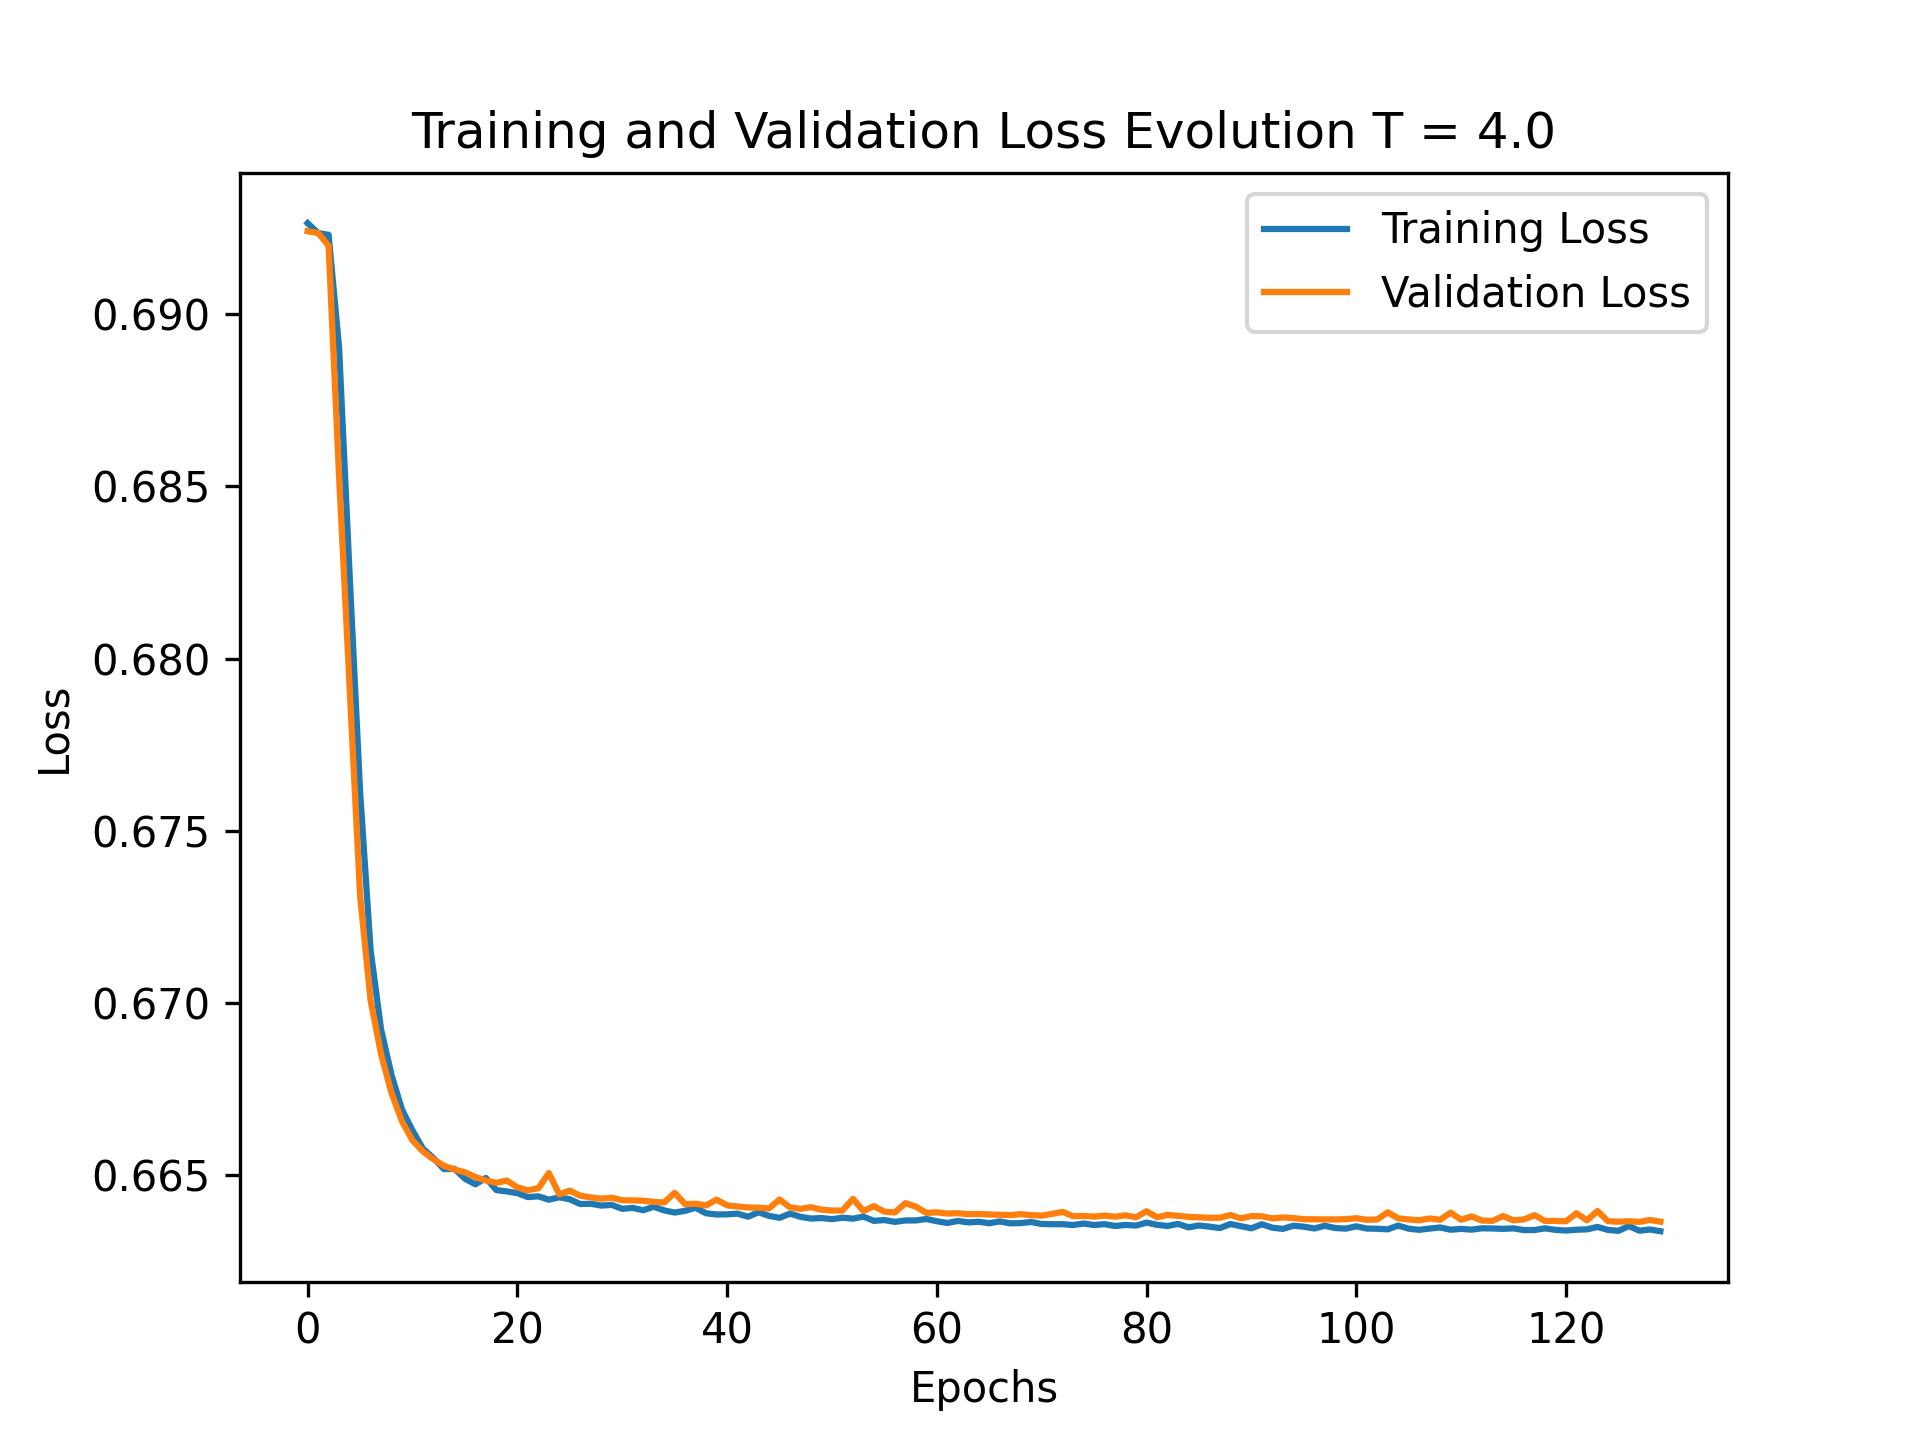
\includegraphics[width=0.9\linewidth]{./figures/evol_T_4.jpg}
		\caption{$T = 4.00$}
		\label{fig:T4}
	\end{subfigure}
	\caption{Convergence des fonction de coûts}
\end{figure}

Une autre méthode pour évaluer la cohérence de l'image de sortie consiste à utiliser les réseaux adversariaux (Adversarial Neural Networks, en anglais).

\subsection{Réseaux Adversariaux}

Cette brève section présente l'une des techniques que nous avons essayées pour surmonter les limites de l'auto-encodeur. Bien qu'elle n'ait pas abouti, nous allons brièvement discuter de son fonctionnement.

Deux réseaux sont entraînés en parallèle. Le premier est un générateur de nouvelles données, chargé de produire des images et des labels. Le deuxième réseau est un discriminateur, dont la mission est de déterminer si une image provient d'un jeu d'entraînement (donc réelle) ou si elle est une image fausse générée par une IA.

À chaque itération, le générateur produit plusieurs images qu'il mélange à un ensemble de données contenant des images réelles. Ensuite, le discriminateur évalue lesquelles sont réelles et lesquelles sont fausses. Une fonction de coût est alors calculée.

Au fil de l'entraînement, les deux réseaux deviennent experts : l'un pour générer de nouvelles images, l'autre pour discerner la subtilité des images générées par rapport aux images réelles. L'entraînement se termine lorsque le discriminateur ne parvient plus à distinguer les images réelles des images produites par l'IA.

Je n'ai pas directement rédigé le programme, mais en utilisant la documentation de TensorFlow sur les réseaux adversariaux, j'ai pu tester ce type d'algorithme qui fonctionne très bien pour le jeu de données MNIST. Cependant, il s'est avéré peu efficace dans notre cas, car il s'agit d'images de bruit ne présentant pas beaucoup de cohérence entre elles.


\newpage
\addcontentsline{toc}{section}{Conclusion}
\section*{Conclusion}

Ce projet a permis d'explorer différentes approches pour comprendre et modéliser le comportement du modèle d'Ising 2D, en mettant en œuvre des méthodes d'intelligence artificielle. L'intérêt principal a été de déterminer la phase du système (paramagnétique ou ferromagnétique) en se basant sur des configurations de spins générées à différentes températures.

\subsection*{Modèle de Magnétisation}

Le modèle basé sur la magnétisation moyenne a montré des performances prometteuses avec une MSE de 0.108, surpassant significativement le modèle naïf. Cependant, il a présenté des difficultés à distinguer les hautes températures, ce qui peut être attribué à la densité de configurations similaires à haute température. Malgré cela, il a réussi à prédire la phase du système avec une précision de 98.8\%, dépassant les attentes initiales.

\subsection*{Modèles d'Apprentissage Profond}

L'utilisation de réseaux de neurones convolutifs (CNN) pour classifier les configurations de spins a été une approche plus complexe. L'entraînement du modèle a nécessité une attention particulière pour éviter le sur-apprentissage en raison du bruit dans les données et du nombre limité de températures distinctes. Cependant, avec un ajustement adéquat des hyperparamètres, le CNN a démontré une capacité à apprendre des caractéristiques complexes et a atteint des performances compétitives.

\subsection*{Génération de Données}

La génération de nouvelles configurations de spins à l'aide d'algorithmes d'Ising et de l'algorithme de Metropolis-Hastings a été réussie. Cela a permis d'élargir le jeu de données pour des températures différentes et d'évaluer la capacité des modèles à généraliser.

\subsection*{Perspectives et Améliorations}

Des améliorations potentielles pourraient inclure l'exploration de modèles plus sophistiqués, la prise en compte de la symétrie du modèle d'Ising dans la conception des architectures de réseaux neuronaux, et l'optimisation plus poussée des hyperparamètres. De plus, l'utilisation d'autres techniques de génération de données, telles que les générateurs adversariaux (GAN), pourrait être envisagée pour créer des configurations de spins plus diversifiées.

En conclusion, ce projet a fourni des insights sur la convergence entre l'intelligence artificielle et la physique, en montrant comment les modèles peuvent être utilisés pour comprendre et classer des phénomènes complexes tels que les transitions de phase dans le modèle d'Ising 2D.

\newpage
\addcontentsline{toc}{section}{Références}
\bibliographystyle{IEEEtran}
\bibliography{bibliographie}
\nocite{noauthor_ising_2023}
\nocite{diu_stat}
\nocite{Ising_auto}

\appendix
\section{Architecture du modèle de CNN} \label{appendix:CNN}
\begin{figure}[H]
	\centering
	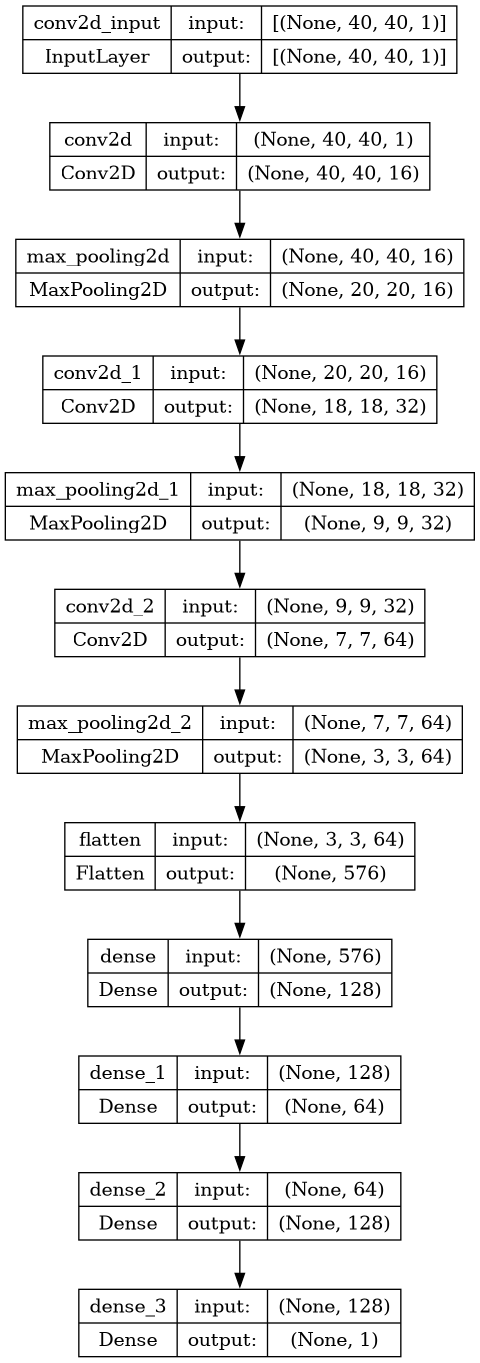
\includegraphics[width=0.48\linewidth]{./figures/model.png}
	\caption{Architecture du modèle}
	\label{fig:model}
\end{figure}

\section{Reconstruction d'image} \label{appendix:reconstruction}
\begin{figure}[H]
	\centering
	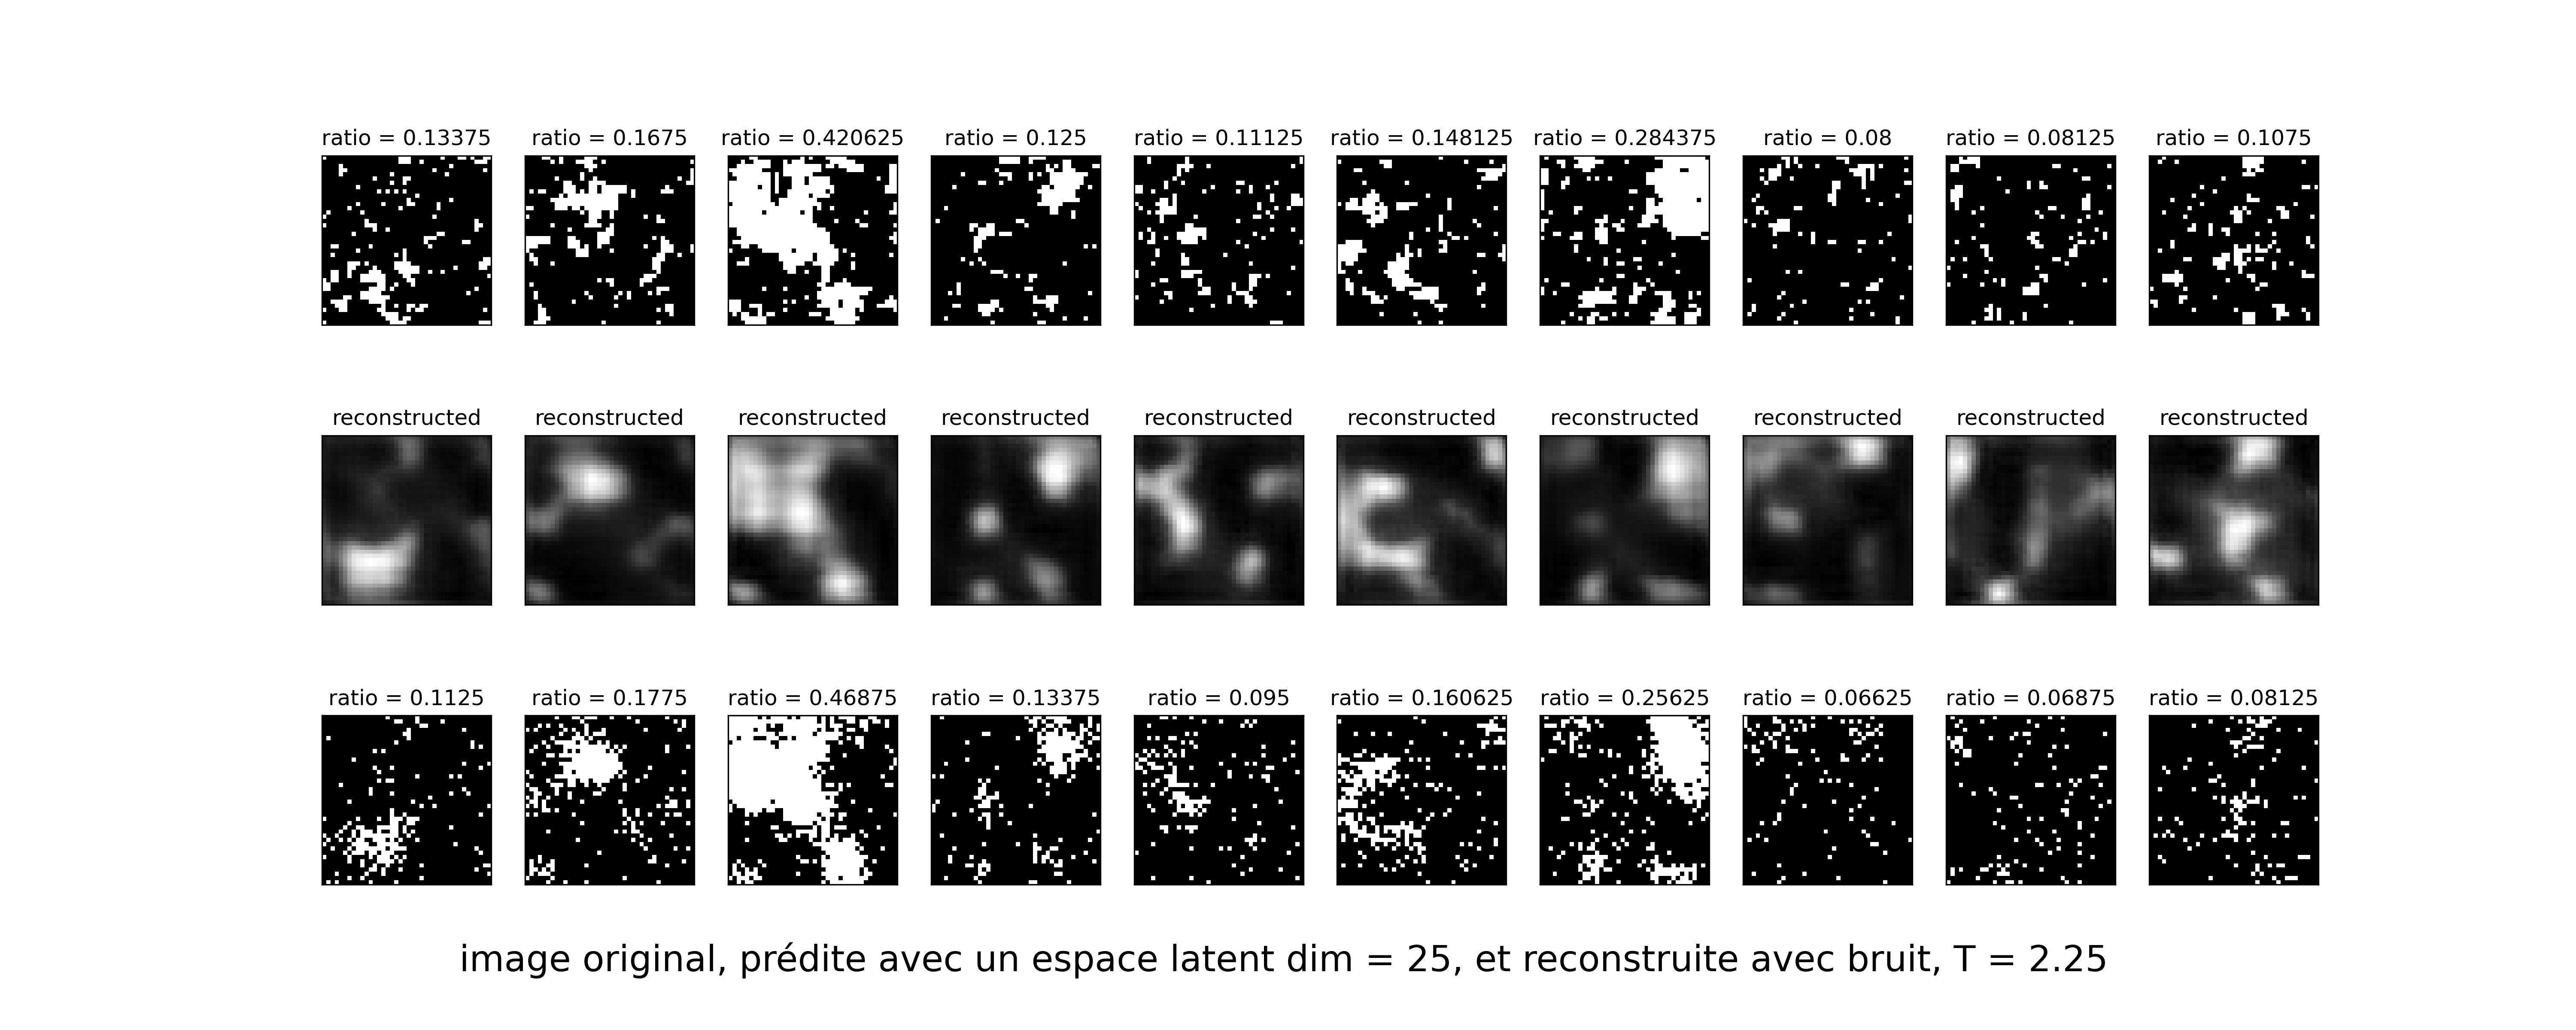
\includegraphics[width=1\linewidth]{./figures/triple.jpg}
	\caption{Reconstruction d'image}
	\label{fig:tiple}
\end{figure}

\end{document}